\newpage
\section{Biểu thức toa độ của các phép toán vectơ}
\subsection{LÝ THUYẾT CẦN NHỚ}
\subsubsection{Biểu thức toạ độ của phép cộng, trừ hai vectơ, phép nhân một số với một vectơ}
\begin{khung4}{}
    Trong không gian $Oxyz$, cho hai vectơ $\overrightarrow{a}=(a_1;a_2;a_3)$ và $\overrightarrow{b}=(b_1;b_2;b_3)$ và số thực $k$. Khi đó:
\begin{itemize}
    \item $\overrightarrow{a}+\overrightarrow{b}=(a_1+b_1;a_2+b_2;a_3+b_3)$;
    \item $\overrightarrow{a}-\overrightarrow{b}=(a_1-b_1;a_2-b_2;a_3-b_3)$;
    \item $k\overrightarrow{a}=(ka_1;ka_2;ka_3)$.
\end{itemize}
\end{khung4}
\begin{nx}
Cho hai vectơ $\overrightarrow{a}=(a_1;a_2;a_3)$ và $\overrightarrow{b}=(b_1;b_2;b_3)$, $\overrightarrow{b} \neq \overrightarrow{0}$. Hai vectơ $\overrightarrow{a}$ và $\overrightarrow{b}$ cùng phương khi và chỉ khi tồn tại số $k$ sao cho $\heva{&a_1=kb_1\\&a_2=kb_2\\&a_3=kb_3.}$
\end{nx}
\subsubsection{Biểu thức toạ độ của tích vô hướng}
\begin{khung4}{}
    Trong không gian $Oxyz$, \indam{tích vô hướng} của hai vectơ $\overrightarrow{a}=(a_1;a_2;a_3)$ và $\overrightarrow{b}=(b_1;b_2;b_3)$ được xác định bỏi công thức
    $$\overrightarrow{a}\cdot \overrightarrow{b}=a_1b_1+a_2b_2+a_3b_3.$$
\end{khung4}
\begin{nx}
    \begin{enumerate}[label=\alph*)]
        \item $\overrightarrow{a} \perp \overrightarrow{b} \Leftrightarrow a_1b_1+a_2b_2+a_3b_3=0$ ($\overrightarrow{a}$, $\overrightarrow{b}$ khác $\overrightarrow{0}$);
        \item $|\overrightarrow{a}|=\sqrt{a_1^2+a_2^2+a_3^2}$;
        \item $\cos(\overrightarrow{a},\overrightarrow{b})=\dfrac{\overrightarrow{a}\cdot \overrightarrow{b}}{|\overrightarrow{a}|\cdot \left|\overrightarrow{b}\right|}=\dfrac{a_1b_1+a_2b_2+a_3b_3}{\sqrt{a_1^2+a_2^2+a_3^2}\cdot \sqrt{b_1^2+b_2^2+b_3^2}}$ ($\overrightarrow{a}$, $\overrightarrow{b}$ khác $\overrightarrow{0}$) . 
    \end{enumerate}
\end{nx}
\subsubsection{Vận dụng}
\begin{khung4}{Xác định toạ độ của vectơ khi biết toạ độ điểm đầu và điểm cuối}
    Trong không gian $Oxyz$, cho hai điểm $A(x_A;y_A;z_A)$, $B(x_B;y_B;z_B)$. Ta có: 
    $$\overrightarrow{AB}=(x_B-x_A;y_B-y_A;z_B-z_A).$$
\end{khung4}
\begin{khung4}{Toạ độ trung điểm của đoạn thẳng và trọng tâm tam giác}
    Trong không gian $Oxyz$:
    \begin{itemize}
        \item Cho hai điểm $A(x_A;y_A;z_A)$, $B(x_B;y_B;z_B)$. Toạ độ trung điểm $M$ của đoạn thẳng $AB$ là:
        $$M\left(\dfrac{x_A+x_B}{2};\dfrac{y_A+y_B}{2};\dfrac{z_A+z_B}{2}\right).$$
        \item Cho tam giác $ABC$ có $A(x_A;y_A;z_A)$, $B(x_B;y_B;z_B)$, $C(x_C;y_C;z_C)$. Toạ độ trọng tâm $G$ của tam giác $ABC$ là:
         $$G\left(\dfrac{x_A+x_B+x_C}{3};\dfrac{y_A+y_B+y_C}{3};\dfrac{z_A+z_B+z_C}{3}\right).$$
    \end{itemize}
\end{khung4}
\subsubsection{Cách tìm toạ độ của một vectơ vuông góc với hai vectơ cho trước}
\begin{khung4}{}
    Cho hai vectơ $\overrightarrow{a}=(a_1;a_2;a_3)$ và $\overrightarrow{b}=(b_1;b_2;b_3)$ không cùng phương. \\
    Khi đó, vectơ $\overrightarrow{c}=(a_2b_3-b_2a_3;a_3b_1-b_3a_1;a_1b_2-b_1a_2)$ vuông góc với cả hai vectơ $\overrightarrow{a}$ và $\overrightarrow{b}$.
\end{khung4}
\begin{nx}
\begin{itemize}
    \item vectơ $\overrightarrow{c}=(a_2b_3-b_2a_3;a_3b_1-b_3a_1;a_1b_2-b_1a_2)$ còn được gọi là \indam{tích có hướng} của hai vectơ $\overrightarrow{a}$ và $\overrightarrow{b}$, kí hiệu là $\overrightarrow{c}=[\overrightarrow{a},\overrightarrow{b}]$.
    \item Để thuận tiện trong cách viết, ta quy ước $\begin{vmatrix}
        a & b \\
        c & d
    \end{vmatrix}$, với $a$, $b$, $c$, $d$ là các số thực. \\
    Khi đó, với hai vectơ $\overrightarrow{a}=(a_1;a_2;a_3)$ và $\overrightarrow{b}=(b_1;b_2;b_3)$, ta có: 
    $$[\overrightarrow{a},\overrightarrow{b}]=\left(\begin{vmatrix}
        a_2 & a_3 \\
        b_2 & b_3
    \end{vmatrix};\begin{vmatrix}
        a_3 & a_1 \\
        b_3 & b_1
    \end{vmatrix};\begin{vmatrix}
        a_1 & a_2 \\
        b_1 & b_2
    \end{vmatrix}\right)=(a_2b_3-b_2a_3;a_3b_1-b_3a_1;a_1b_2-b_1a_2).$$
    \item Hai vectơ $\overrightarrow{a}$, $\overrightarrow{b}$ không cùng phương khi và chỉ khi vectơ $\overrightarrow{c}=[\overrightarrow{a},\overrightarrow{b}]\neq \overrightarrow{0}$.
\end{itemize}
\end{nx}
\subsection{PHÂN LOẠI VÀ PHƯƠNG PHÁP GIẢI TOÁN}
\begin{dang}{Tìm toạ độ vectơ}
Ta sử dụng tính chất tổng, hiệu hai vectơ và tích một số với một vectơ.
\end{dang}

\begin{vd}%[2H2H2-3]%[Dự án dề cương 3 Khối NH24-25-Đợt 2-Nguyễn Thanh Phong]
Trong không gian với hệ toạ độ $Oxyz$ cho $\overrightarrow{a}=(-1;2;3)$, $\overrightarrow{b}=(3;1;-2)$, $\overrightarrow{c}=(4;2;-3)$.
\begin{enumerate}[label=\alph*)]
    \item Tìm toạ độ vectơ $\overrightarrow{u}=2\overrightarrow{a}+\overrightarrow{b}-3\overrightarrow{c}$.
    \item Tìm toạ độ vectơ $\overrightarrow{v}+2\overrightarrow{b}=\overrightarrow{a}+\overrightarrow{c}$.
\end{enumerate}
\loigiai{
\begin{enumerate}[label=\alph*)]
    \item Ta có $2\overrightarrow{a} = (-2; 4; 6)$ và $\overrightarrow{b} = (3; 1; -2)$. Do đó, $2\overrightarrow{a} + \overrightarrow{b} = (-2 + 3; 4 + 1; 6 + (-2))$ hay $2\overrightarrow{a} + \overrightarrow{b} = (1; 5; 4)$. Ngoài ra, vì $3\overrightarrow{c} = (12; 6; -9)$ nên $\overrightarrow{u} = 2\overrightarrow{a} + \overrightarrow{b} - 3\overrightarrow{c} = (-11; -1; 13)$.
    
    \item Ta có $2\overrightarrow{b} = (6; 2; -4)$. Gọi $\overrightarrow{v} = (x; y; z)$, khi đó $\overrightarrow{v} + 2\overrightarrow{b} = (x + 6; y + 2; z - 4)$, $\overrightarrow{a} + \overrightarrow{c} = (-1 + 4; 2 + 2; 3 - 3)$ hay $\overrightarrow{a} + \overrightarrow{c} = (3; 4; 0)$. Do đó, $\overrightarrow{v} + 2\overrightarrow{b} = \overrightarrow{a} + \overrightarrow{c}$ khi và chỉ khi
    $$
    \heva{
        &x + 6 = 3 \\
        &y + 2 = 4 \\
        &z - 4 = 0
    }
    \Leftrightarrow
    \heva{
       & x = -3 \\
       & y = 2 \\
       & z = 4.
    }
    $$
    Vậy tọa độ của $\overrightarrow{v} = (-3; 2; 4)$.
\end{enumerate}
}
\end{vd}


\begin{vd}%[2H2H2-5]%[Dự án dề cương 3 Khối NH24-25-Đợt 2-Nguyễn Thanh Phong]
Trong không gian với hệ tọa độ $Oxyz$, cho $\overrightarrow{a} = (2; -2; 1)$, $\overrightarrow{b} = (2; 1; 3)$. Hãy chỉ ra tọa độ của một vectơ $\overrightarrow{c}$ khác vectơ $\overrightarrow{0}$ vuông góc với cả hai vectơ $\overrightarrow{a}$ và $\overrightarrow{b}$.
\loigiai{
    Ta có $\overrightarrow{c} = [\overrightarrow{a}, \overrightarrow{b}] = (-7; -4; 6)$. Mà $\overrightarrow{a} \cdot \overrightarrow{c} = 0$ và $\overrightarrow{b} \cdot \overrightarrow{c} = 0$. Nên khi đó vectơ $\overrightarrow{c}$ vuông góc với hai vectơ $\overrightarrow{a}$ và $\overrightarrow{b}$.
}
\end{vd}


\begin{vd}%[2H2H2-5]%[Dự án dề cương 3 Khối NH24-25-Đợt 2-Nguyễn Thanh Phong]
    Cho hình hộp $ABCD.A'B'C'D'$ biết $A(1; 0; 1)$, $B(2; 1; 2)$, $D(1; -1; 1)$, $C'(4; 5; -5)$. Hãy chỉ ra tọa độ của một vectơ vuông góc với cả hai vectơ trong mỗi trường hợp sau:
\begin{enumerate}[label=\alph*)]
    \item $\overrightarrow{AC}$ và $\overrightarrow{B'D'}$;
    \item $\overrightarrow{AC'}$ và $\overrightarrow{BD}$.
\end{enumerate}
\loigiai{
\begin{enumerate}[label=\alph*)]
    \item Ta có: $\overrightarrow{AB} = (1; 1; 1)$. Gọi tọa độ của điểm $C$ là $(x_C; y_C; z_C)$, ta có:
    $\overrightarrow{DC} = (x_C - 1; y_C + 1; z_C - 1)$. Trong hình hộp $ABCD.A'B'C'D'$, ta có: $\overrightarrow{AB} = \overrightarrow{DC}$.
    
    Suy ra: 
    $\heva{
        x_C - 1 = 1 \\
        y_C + 1 = 1 \\
        z_C - 1 = 1
    }
    \Leftrightarrow
    \heva{
        x_C = 2 \\
        y_C = 0 \\
        z_C = 2.
    }$
    
    Vậy tọa độ của điểm $C(2; 0; 2)$.
    
    Tương tự, ta có: $D'(3; 4; -6)$, $B'(4; 6; -5)$.
    
    $\overrightarrow{AC} = (1; 0; 1)$ và $\overrightarrow{B'D'} = (-1; -2; -1)$. Khi đó, $\overrightarrow{u} = [\overrightarrow{AC}, \overrightarrow{B'D'}] = (2; 0; -2)$.
    
    Vậy $\overrightarrow{u} = (2; 0; -2)$ vuông góc với hai vectơ $\overrightarrow{AC}$ và $\overrightarrow{B'D'}$.

    \item Ta có: $\overrightarrow{AC'} = (3; 5; -6)$, $\overrightarrow{BD} = (-1; -2; -1)$.
    
    Khi đó, $\overrightarrow{v} = [\overrightarrow{AC'}, \overrightarrow{BD}] = (-17; 9; -1)$. Vậy vectơ $\overrightarrow{v} = (-17; 9; -1)$ vuông góc với hai vectơ $\overrightarrow{AC'}$ và $\overrightarrow{BD}$.
\end{enumerate}
}
\end{vd}
\begin{dang}{Tìm toạ độ điểm}
    Sử dụng các tính chất về trung điểm, trọng tâm để tìm toạ độ của điểm.
\end{dang}
\begin{vd}%[2H2H2-2]%[Dự án dề cương 3 Khối NH24-25-Đợt 2-Nguyễn Thanh Phong]
    Trong không gian với hệ toạ độ $Oxyz$, cho $M(-2;3;1)$, $N(4;0;3)$. Tìm toạ độ của điểm $P$ để $N$ là trung điểm của đoạn thẳng $MP$.
\loigiai{
Gọi tọa độ của điểm $P$ là $(x_P ; y_P ; z_P)$. Vì $N$ là trung điểm của đoạn thẳng $MP$ nên ta có:
$$
\heva{
    &x_N = \dfrac{x_M + x_P}{2} \\
    &y_N = \dfrac{y_M + y_P}{2} \\
    &z_N = \dfrac{z_M + z_P}{2}
}
\Leftrightarrow
\heva{
    &x_P = 2x_N - x_M \\
    &y_P = 2y_N - y_M \\
    &z_P = 2z_N - z_M
}
\Leftrightarrow
\heva{
    &x_P = 10 \\
    &y_P = -3 \\
    &z_P = 5.
}
\Rightarrow P(10;-3;5).
$$
}
\end{vd}
\begin{vd}%[2H2H2-2]%[Dự án dề cương 3 Khối NH24-25-Đợt 2-Nguyễn Thanh Phong]
Trong không gian với hệ tọa độ $Oxyz$, cho tam giác $ABC$ có $A(1; 0; 1)$, $B(2; 1; 2)$ và trọng tâm $G(1; -1; 1)$. Tìm tọa độ của đỉnh $C$.
\loigiai{
Gọi tọa độ của điểm $C$ là $(x_C; y_C; z_C)$. Vì $G$ là trọng tâm của tam giác $ABC$, ta có:
\[
\heva{
    &x_G = \dfrac{x_A + x_B + x_C}{3} \\
    &y_G = \dfrac{y_A + y_B + y_C}{3} \\
    &z_G = \dfrac{z_A + z_B + z_C}{3}
}
\Leftrightarrow
\heva{
    &x_C = 3x_G - x_A - x_B \\
    &y_C = 3y_G - y_A - y_B \\
    &z_C = 3z_G - z_A - z_B
}
\Leftrightarrow
\heva{
    &x_C = 0 \\
    &y_C = -4 \\
    &z_C = 0.
}
\]
Vậy tọa độ của điểm $C(0; -4; 0)$.
}
\end{vd}
\begin{dang}{Tích vô hướng và các ứng dụng của tích vô hướng}
Áp dụng công thức tính tích vô hướng và các tính chất liên quan đến góc.
\end{dang}
\begin{vd}%[2H2H2-5]%[Dự án dề cương 3 Khối NH24-25-Đợt 2-Nguyễn Thanh Phong]
Trong không gian với hệ tọa độ $Oxyz$, cho $\overrightarrow{a} = (3; 2; -1)$, $\overrightarrow{b} = (-2; 1; 2)$.
Tính côsin của góc $(\overrightarrow{a}, \overrightarrow{b})$.
\loigiai{
Côsin của góc $(\overrightarrow{a}, \overrightarrow{b})$ là:
\[
\cos(\overrightarrow{a}, \overrightarrow{b}) = \dfrac{\overrightarrow{a} \cdot \overrightarrow{b}}{|\overrightarrow{a}|.\left|\overrightarrow{b}\right|} = \dfrac{3 . (-2) + 2 . 1 + (-1) . 2}{\sqrt{3^2 + 2^2 + (-1)^2} . \sqrt{(-2)^2 + 1^2 + 2^2}} = \dfrac{-2}{\sqrt{14}}.
\]
}
\end{vd}
\begin{dang}{Ứng dụng}
    Vận dụng các kiến thức, tính chất ở trên để giải quyết các bài toán thực tế.
\end{dang}
\begin{vd}%[2H2H2-6] %[Lớp 12 – Đề thi học kì 1]%[Thanh Phát]
	Hai chiếc flycam được điều khiển cùng bay lên tại một địa điểm. Sau một thời gian bay, chiếc flycam thứ nhất ở vị trí $A$ cách mặt đất $3\,$m, cách điểm xuất phát $3\,$m về phía Nam và $2\,$m về phía Đông. Chiếc flycam thứ hai ở vị trí $B$ cách mặt đất $5\,$m, cách điểm xuất phát $2\,$m về phía Bắc và $4\,$m về phía Tây. Chọn hệ trục tọa độ $Oxyz$ với gốc $O$ đặt tại điểm xuất phát của hai chiếc flycam, mặt phẳng $(Oxy)$ trùng với mặt đất có trục $Ox$ hướng về phía Nam, trục $Oy$ hướng về phía Đông và trục $Oz$ hướng thẳng đứng lên trời (đơn vị lấy theo mét). Gọi $M(a;b;c)$ là một điểm nằm trên mặt đất sao cho ba điểm $M$, $A$, $B$ thẳng hàng. Khi đó $2a+b+c$ bằng?
	\loigiai{Từ cách đặt hệ trục tọa độ $Oxyz$, ta có $A(3;2;3)$, $B(-2;-4;5)$.\\
		Vì $M$ thuộc mặt đất nên $M(a;b;0)$ $(c=0)$. \\
		Ta có $\overrightarrow{AM}=(a-3;b-2;-3)$, $\overrightarrow{AB}=(-5;-6;2)$.\\
		Ta có $A$, $B$, $M$ thẳng hàng nên $\overrightarrow{AM}$, $\overrightarrow{AB}$ cùng phương
		\begin{eqnarray*}
			&\Leftrightarrow &\dfrac{a-3}{-5} = \dfrac{b-2}{-6} = \dfrac{-3}{2}\\
			&\Leftrightarrow &\heva{&a=\dfrac{21}{2} \\
				&b=11.}
		\end{eqnarray*}
		Vậy $2a+b+c= 2\cdot \dfrac{21}{2} + 11 +0 =32$.
	}
\end{vd}
\subsection{Bài tập rèn luyện}
\ind{PHẦN I.} \inden{Câu trắc nghiệm nhiều phương án lựa chọn. Mỗi câu hỏi học sinh chỉ chọn một phương án.}\\
\setcounter{ex}{0}
\Opensolutionfile{ans}[ans/2H2-Bai3-TN]%--Đặt tên 2H2-Bai3-Dang1-TN
%%%%%%%%%%%%%%%%%%%%%%%%%%%%%%%%%%%%%%%%%%%%%%%%%%%%%%%%%
% BẮT ĐẦU PHẦN 1: CÂU HỎI MỨC ĐỘ NHẬN BIẾT (N)
%%%%%%%%%%%%%%%%%%%%%%%%%%%%%%%%%%%%%%%%%%%%%%%%%%%%%%%%%

%============Câu 1=======================
\begin{ex}%[2H2N2-3]%[Dự án dề cương 3 Khối NH24-25-Đợt 2-Nguyễn Thanh Phong]
	\textit{(Trích đề thi HKI - Trường THPT Phan Bội Châu - Khánh Hoà - Năm học 2024 - 2025)} \\
	Trong không gian với hệ trục tọa độ $Oxyz$, cho hai vectơ $\overrightarrow{a}=(-2;5;-3)$ và $\overrightarrow{w}=(4;-4;-6)$. Tọa độ vectơ $-2\overrightarrow{a}-3\overrightarrow{w}$ là
\choice
{$(8;-19;0)$}
{$(2;1;-9)$}
{\True $(-8;2;24)$}
{$(10;2;15)$}
\loigiai{Gọi $\overrightarrow{u}=-2\overrightarrow{a}-3\overrightarrow{w}=-2(-2;5;-3)-3(4;-4;-6)=(4;-10;6)-(12;-12;-18)=(-8;2;24)$.
}
\end{ex}
%============Câu 2=======================
\begin{ex}%[2H2N2-3]%[Dự án dề cương 3 Khối NH24-25-Đợt 2-Nguyễn Thanh Phong]
	\textit{(Trích đề thi HKI - Trường THPT Phan Bội Châu - Khánh Hoà - Năm học 2024 - 2025)} \\
	Trong không gian với hệ tọa độ $Oxyz$, cho hai điểm $C(-1;-8;-10)$ và $Q(-6;-1;-3)$. Tọa độ của vectơ $\overrightarrow{CQ}$ là
\choice
{\True $(-5;7;7)$}
{$(6;8;30)$}
{$(5;-7;-7)$}
{$(-7;-9;-13)$}
\loigiai{Ta có: $\overrightarrow{CQ}=(-6-(-1);-1-(-8);-3-(-10))=(-5;7;7)$.
}
\end{ex}
%============Câu 3======================
\begin{ex}%[2H2N2-3]%[Dự án dề cương 3 Khối NH24-25-Đợt 2-Nguyễn Thanh Phong]
	\textit{(Trích đề thi HKI - Trường THPT Chuyên Lê Thánh Tông - Quảng Nam - Năm học 2024 - 2025)} \\
	Trong không gian với hệ tọa độ $Oxyz$, cho hai điểm $P(2;0;-1)$, $Q(1;-1;3)$. Tọa độ vectơ $\overrightarrow{PQ}$ là
\choice
{$\overrightarrow{PQ}(2;0;-1)$}
{\True $\overrightarrow{PQ}(-1;-1;4)$}
{$\overrightarrow{PQ}(1;-1;3)$}
{$\overrightarrow{PQ}(1;1;-4)$}
\loigiai{Ta có: $\overrightarrow{PQ}=(1-2;-1-0;3-(-1))=(-1;-1;4)$.
}
\end{ex}
%============Câu 4=======================
\begin{ex}%[2H2N2-2]%[Dự án dề cương 3 Khối NH24-25-Đợt 2-Nguyễn Thanh Phong]
	\textit{(Trích đề thi HKI - Trường THPT Phan Bội Châu - Khánh Hoà - Năm học 2024 - 2025)} \\
	Trong không gian với hệ tọa độ $Oxyz$, cho điểm $A(-8;8;2)$ và vectơ $\overrightarrow{a}=(-12;5;-15)$. Biết rằng $\overrightarrow{AD}=\overrightarrow{a}$, tọa độ điểm $D$ là
\choice
{$(-4;-3;-17)$}
{$(4;3;17)$}
{\True $(-20;13;-13)$}
{$(-20;-3;-17)$}
\loigiai{Gọi $D(x_D;y_D;z_D)$.\\
Ta có: $\overrightarrow{AD}=(x_D-(-8);y_D-8;z_D-2)=(-12;5;-15)$ suy ra $\heva{&x_D-(-8)=-12\\&y_D-8=5\\&z_D-2=-15} \Rightarrow \heva{&x_D=-20\\&y_D=13\\&z_D=-13.}$\\
 Do đó, $D(-20;13;-13)$.
}
\end{ex}
%============Câu 5=======================
\begin{ex}%[2H2N2-2]%[Dự án dề cương 3 Khối NH24-25-Đợt 2-Nguyễn Thanh Phong]
	\textit{(Trích đề thi HKI - Trường THPT Chuyên Lê Thánh Tông - Quảng Nam - Năm học 2024 - 2025)} \\
	Trong không gian $Oxyz$, cho hai điểm $A$, $B$ với $A(1;2;-4)$ và $\overrightarrow{AB}=(-4;0;6)$. Tọa độ của điểm $B$ là
\choice
{$(-1;6;-6)$}
{$(5;2;-10)$}
{\True $(-3;2;2)$}
{$(0;4;-5)$}
\loigiai{Gọi $B(x_B;y_B;z_B)$.\\
Ta có: $\overrightarrow{AB}=(x_B-1;y_B-2;z_B-(-4))=(-4;0;6)$ suy ra $\heva{&x_B-1=-4\\&y_B-2=0\\&z_B-(-4)=6}\Rightarrow \heva{&x_B=-3\\&y_B=2\\&z_B=2.}$\\
 Do đó, $B(-3;2;2)$.
}
\end{ex}
%============Câu 6=======================
\begin{ex}%[2H2N2-2]%[Dự án dề cương 3 Khối NH24-25-Đợt 2-Nguyễn Thanh Phong]
	\textit{(Trích đề thi HKI - Trường THPT Thực hành Sư Phạm - Đồng Nai - Năm học 2024 - 2025)} \\
	Trong không gian $Oxyz$, cho $\overrightarrow{MO}=-\overrightarrow{i}+2\overrightarrow{j}-2\overrightarrow{k}$ và $N(1;0;4)$. Tọa độ trung điểm của đoạn thẳng $MN$ là
\choice
{$(0;1;1)$}
{$(1;0;3)$}
{\True $(1;-1;3)$}
{$(2;-2;6)$}
\loigiai{
\begin{itemize}
    \item Gọi $M(x_M; y_M; z_M)$, có $O(0;0;0)$.
    \item Ta có $\overrightarrow{MO} = (0 - x_M; 0 - y_M; 0 - z_M) = (-1; 2; -2)$.
    \item Suy ra $\heva{&0 - x_M = -1 \\ &0 - y_M = 2 \\ &0 - z_M = -2} \Rightarrow \heva{&x_M = 1 \\&y_M = -2 \\&z_M = 2.}$
    \item Do đó $M(1; -2; 2)$.
    \item Gọi $I(x_I; y_I; z_I)$ là trung điểm của đoạn thẳng $MN$ nên ta có:
$$\heva{&x_I = \dfrac{x_M + x_N}{2} \\&y_I = \dfrac{y_M + y_N}{2} \\&z_I = \dfrac{z_M + z_N}{2}} \Leftrightarrow \heva{&x_I = \dfrac{1+1}{2} = 1 \\&y_I = \dfrac{-2+0}{2} = -1 \\&z_I = \dfrac{2+4}{2} = 3.}$$
    \item Do đó tọa độ trung điểm $MN$ là $(1; -1; 3)$.
\end{itemize}
}
\end{ex}
%============Câu 7=======================
\begin{ex}%[2H2N2-2]%[Dự án dề cương 3 Khối NH24-25-Đợt 2-Nguyễn Thanh Phong]
	Trong không gian với hệ tọa độ $Oxyz$, cho hai điểm $A(2;1;1)$ và $B(-1;2;1)$. Tìm tọa độ điểm $A'$ đối xứng với $A$ qua điểm $B$.
\choice
{$A'(3;4;-3)$}
{\True $A'(-4;3;1)$}
{$A'(1;3;2)$}
{$A'(5;0;1)$}
\loigiai{
\begin{itemize}
    \item Gọi $A'$($x_{A'}$, $y_{A'}$, $z_{A'}$) là điểm đối xứng với $A$ qua $B$ $\Rightarrow$ $B$ là trung điểm của $AA'$.
    \item Ta có $\heva{&x_B = \dfrac{x_A + x_{A'}}{2} \\&y_B = \dfrac{y_A + y_{A'}}{2} \\&z_B = \dfrac{z_A + z_{A'}}{2}} \Leftrightarrow \heva{&x_{A'} = 2x_B - x_A \\&y_{A'} = 2y_B - y_A \\&z_{A'} = 2z_B - z_A} \Leftrightarrow \heva{&x_{A'} = -4 \\&y_{A'} = 3 \\&z_{A'} = 1.} $
    \item Do đó $A'(-4; 3; 1)$.
\end{itemize}
}
\end{ex}
%============Câu 8=======================
\begin{ex}%[2H2N2-2]%[Dự án dề cương 3 Khối NH24-25-Đợt 2-Nguyễn Thanh Phong]
	Trong không gian $Oxyz$, cho hai điểm $A(1;3;2)$ và $B(3;1;0)$. Điểm $C$ đối xứng với $A$ qua $B$ có tọa độ là
\choice
{$(2;2;-1)$}
{$(5;-1;2)$}
{$(2;2;1)$}
{\True $(5;-1;-2)$}
\loigiai{
\begin{itemize}
    \item Gọi $C(x_C; y_C; z_C)$ là điểm đối xứng của $A$ qua $B$ $\Rightarrow$ $B$ là trung điểm của $AC$.
    \item Ta có $\heva{&x_B = \dfrac{x_A+x_C}{2} \\&y_B = \dfrac{y_A+y_C}{2} \\&z_B = \dfrac{z_A+z_C}{2}} \Leftrightarrow \heva{&x_C = 2x_B - x_A \\&y_C = 2y_B - y_A \\&z_C = 2z_B - z_A}    \Leftrightarrow \heva{&x_C = 5 \\&y_C = -1 \\&z_C = -2.}$
    \item Do đó $C(5; -1; -2)$.
\end{itemize}
}
\end{ex}
%============Câu 9=======================
\begin{ex}%[2H2N2-3]%[Dự án dề cương 3 Khối NH24-25-Đợt 2-Nguyễn Thanh Phong]
	Trong không gian với hệ tọa độ $Oxyz$, cho điểm $A(2;2;1)$; $B(0;-1;2)$. Tính độ dài đoạn thẳng $AB$.
\choice
{$AB=2\sqrt{3}$}
{\True $AB=\sqrt{14}$}
{$AB=\sqrt{13}$}
{$AB=\sqrt{6}$}
\loigiai{
\begin{itemize}
    \item Ta có $\overrightarrow{AB} = (-2; -3; 1)$ có $AB = |\overrightarrow{AB}| = \sqrt{(-2)^2 + (-3)^2 + 1^2} = \sqrt{14}$.
    \item Vậy độ dài đoạn $AB = \sqrt{14}$.
\end{itemize}
}
\end{ex}
%============Câu 10=======================
\begin{ex}%[2H2N2-3]%[Dự án dề cương 3 Khối NH24-25-Đợt 2-Nguyễn Thanh Phong]
	Trong không gian với hệ tọa độ $Oxyz$, cho điểm $M(2;-1;2)$. Tính độ dài đoạn thẳng $OM$.
\choice
{$OM = \sqrt{5}$}
{$OM = 9$}
{$OM = \sqrt{3}$}
{\True $OM = 3$}
\loigiai{
\begin{itemize}
    \item Ta có $M(2; -1; 2)$, $O(0; 0; 0)$ $\Rightarrow \overrightarrow{OM} = (2, -1, 2)$. Ta tính: $OM = |\overrightarrow{OM}| = \sqrt{2^2 + (-1)^2 + 2^2} = 3$.
    \item Vậy độ dài đoạn $OM = 3$.
\end{itemize}
}
\end{ex}
%============Câu 11=======================
\begin{ex}%[2H2N2-2]%[Dự án dề cương 3 Khối NH24-25-Đợt 2-Nguyễn Thanh Phong]
	Trong không gian $Oxyz$, cho tam giác $BCD$ với $B(3;2;-5)$, $C(-1;0;2)$, $D(7;4;0)$. Tọa độ trọng tâm của tam giác $BCD$ là
\choice
{\True $(3;2;-1)$}
{$(9;6;-3)$}
{$(3;-1;2)$}
{$(3;-2;-1)$}
\loigiai{
\begin{itemize}
    \item Gọi $I(x_I; y_I; z_I)$ là tọa độ trọng tâm của $\triangle BCD$.
    \item Ta có $\heva{&x_I = \dfrac{x_B + x_C + x_D}{3} \\&y_I = \dfrac{y_B + y_C + y_D}{3} \\&z_I = \dfrac{z_B + z_C + z_D}{3}} \Leftrightarrow \heva{&x_I = \dfrac{3 - 1 + 7}{3}=3 \\&y_I = \dfrac{2 + 0 + 4}{3}=2 \\&z_I = \dfrac{-5 + 2 + 0}{3}=-1}\Rightarrow I(3; 2; -1)$.
\end{itemize}
}
\end{ex}
%============Câu 12=======================
\begin{ex}%[2H2N2-4]%[Dự án dề cương 3 Khối NH24-25-Đợt 2-Nguyễn Thanh Phong]
	Trong không gian $Oxyz$, cho $A(1;-2;3)$, $B(2;-4;1)$, $C(2;0;2)$, khi đó tích vô hướng $\overrightarrow{AB} \cdot \overrightarrow{AC}$ bằng
\choice
{$7$}
{$-5$}
{$4$}
{\True $-1$}
\loigiai{
\begin{itemize}
    \item Ta có $\overrightarrow{AB} = (1; -2; -2)$, $\overrightarrow{AC} = (1; 2; -1)$.
    \item Vậy $\overrightarrow{AB} \cdot \overrightarrow{AC} = 1 \cdot 1 + (-2) \cdot 2 + (-2) \cdot (-1) = 1 - 4 + 2= -1$.
\end{itemize}
}
\end{ex}

%============Câu 13======================
\begin{ex}%[2H2H2-4]%[Dự án dề cương 3 Khối NH24-25-Đợt 2-Nguyễn Thanh Phong]
	\textit{(Trích đề thi HKI - Trường THPT Chuyên Lê Thánh Tông - Quảng Nam - Năm học 2024 - 2025)} \\
	Trong không gian $Oxyz$, cho vectơ $\overrightarrow{a}=(1;2;0)$, $\overrightarrow{b}=(-1;1;2)$. Biểu thức $2\overrightarrow{a}(\overrightarrow{a}+2\overrightarrow{b})$ bằng:
\choice
{$-8$}
{$30$}
{$1$}
{\True $14$}
\loigiai{
\begin{itemize}
    \item Ta có: $\overrightarrow{a} + 2\overrightarrow{b} = (1+2\cdot(-1); 2+2\cdot1; 0+2\cdot2) = (-1; 4; 4)$, $2\overrightarrow{a} = (2\cdot 1; 2\cdot 2; 2\cdot 0) = (2; 4; 0)$.
    \item Vậy $2\overrightarrow{a}(\overrightarrow{a} + 2\overrightarrow{b}) = (-1)\cdot 2 + 4\cdot 4 + 0\cdot 4 = -2 + 16 = 14$.
\end{itemize}
}
\end{ex}
%============Câu 14=======================
\begin{ex}%[2H2H2-6]%[Dự án dề cương 3 Khối NH24-25-Đợt 2-Nguyễn Thanh Phong]
	Trong không gian với hệ tọa độ $Oxyz$, cho điểm $A(4;0;0)$, $B(0;2;0)$. Tâm đường tròn ngoại tiếp tam giác $OAB$ là
\choice
{$I(2;-1;0)$}
{$I\left(\dfrac{4}{3};\dfrac{2}{3};0\right)$}
{$I(-2;1;0)$}
{\True $I(2;1;0)$}
\loigiai{
\begin{itemize}
    \item Ta có $A(4; 0; 0) \in Ox$, $B(0; 2; 0) \in Oy$ $\Rightarrow \triangle OAB$ vuông tại $O$.
    \item Do đó, tâm đường tròn ngoại tiếp $\triangle OAB$ là trung điểm của $AB$.
    \item Gọi $I$ là trung điểm $AB$, ta tính: $\heva{&x_I = \dfrac{x_A + x_B}{2} \\&y_I = \dfrac{y_A + y_B}{2} \\&z_I = \dfrac{z_A + z_B}{2}} \Rightarrow \heva{&x_I = 2 \\&y_I = 1 \\&z_I = 0.}$
    \item Vậy tâm đường tròn ngoại tiếp $OAB$ có tọa độ $I(2; 1; 0)$.
\end{itemize}
}
\end{ex}
%============Câu 15=======================
\begin{ex}%[2H2H2-2]%[Dự án dề cương 3 Khối NH24-25-Đợt 2-Nguyễn Thanh Phong]
	Trong không gian $Oxyz$, cho tam giác $ABC$ có trọng tâm $G(-3;1;4)$ và $A(1;0;-1)$, $B(2;3;5)$. Tọa độ điểm $C$ là
\choice
{$C(-6;2;0)$}
{$C(4;2;-1)$}
{\True $C(-12;0;8)$}
{$C(3;-1;-5)$}
\loigiai{
\begin{itemize}
    \item Gọi tọa độ điểm $C$ là $(x_C; y_C; z_C)$.
    \item Vì $G$ là trọng tâm của $\triangle ABC$, ta có:
    \item $\heva{&x_G = \dfrac{x_A + x_B + x_C}{3} \\&y_G = \dfrac{y_A + y_B + y_C}{3} \\&z_G = \dfrac{z_A + z_B + z_C}{3}.} \Leftrightarrow \heva{&x_C = 3x_G - x_A - x_B \\&y_C = 3y_G - y_A - y_B \\&z_C = 3z_G - z_A - z_B}\Leftrightarrow \heva{&x_c = -12 \\&y_c = 0 \\&z_c = 8.}$
    \item Vậy tọa độ điểm $C$ $(-12; 0; 8)$.
\end{itemize}
}
\end{ex}
%============Câu 16=======================
\begin{ex}%[2H2H2-6]%[Dự án dề cương 3 Khối NH24-25-Đợt 2-Nguyễn Thanh Phong]
	Trong không gian với hệ trục tọa độ $Oxyz$, cho tam giác $ABC$ với $\overrightarrow{AB}=(1;-2;2)$, $\overrightarrow{AC}=(3;-4;6)$. Độ dài đường trung tuyến $AM$ của tam giác $ABC$ là
\choice
{$\dfrac{\sqrt{29}}{2}$}
{$29$}
{\True $\sqrt{29}$}
{$2\sqrt{29}$}
\loigiai{
\begin{itemize}
	\item Ta có: $\overrightarrow{AM}=\dfrac{1}{2}(\overrightarrow{AB}+\overrightarrow{AC})=\dfrac{1}{2}[(1;-2;2)+(3;-4;6)]=(2;-3;4)$.
    \item Ta có $AM = |\overrightarrow{AM}| = \sqrt{2^2 + (-3)^2 + 4^2} = \sqrt{29}$.
    \item Vậy độ dài đường trung tuyến $AM$ bằng $\sqrt{29}$.
\end{itemize}
}
\end{ex}
%============Câu 17=======================
\begin{ex}%[2H2H2-6]%[Dự án dề cương 3 Khối NH24-25-Đợt 2-Nguyễn Thanh Phong]
	Cho tam giác $ABC$ biết $A(2;-1;3)$ và trọng tâm $G(2;1;0)$. Khi đó $\overrightarrow{AB}+\overrightarrow{AC}$ có tọa độ là
\choice
{$(0;6;9)$}
{$(0;9;-9)$}
{$(0;-9;9)$}
{\True $(0;6;-9)$}
\loigiai{
Ta có: 
\begin{align*}
	\overrightarrow{AB} + \overrightarrow{AC} &= \overrightarrow{AG} + \overrightarrow{GB} + \overrightarrow{AG} + \overrightarrow{GC}\\
	&= \overrightarrow{AG} + \overrightarrow{GB} + \overrightarrow{AG} + \overrightarrow{GC} + \overrightarrow{AG} + \overrightarrow{GA} \quad (\text{Vì } \overrightarrow{AG} + \overrightarrow{GA} = \overrightarrow{0})\\
	&= 3\overrightarrow{AG} + (\overrightarrow{GA}+\overrightarrow{GB}+\overrightarrow{GC})\\
	&=3\overrightarrow{AG}\\
	&=3\cdot (2-2;1-(-1);0-3) = (0;6;-9).
\end{align*}

}
\end{ex}
%============Câu 18=======================
\begin{ex}%[2H2H2-4]%[Dự án dề cương 3 Khối NH24-25-Đợt 2-Nguyễn Thanh Phong]
	Trong không gian với hệ trục tọa độ $Oxyz$, cho hai vectơ $\overrightarrow{a}=(3;-2;m)$, $\overrightarrow{b}=(2;m;-1)$ với $m$ là tham số nhận giá trị thực. Tìm giá trị của $m$ để hai vectơ $\overrightarrow{a}$ và $\overrightarrow{b}$ vuông góc với nhau.
\choice
{$m=-2$}
{$m=-1$}
{\True $m=2$}
{$m=1$}
\loigiai{
Để $\overrightarrow{a} \perp \overrightarrow{b}$ thì $\overrightarrow{a} \cdot \overrightarrow{b} = 0 \Leftrightarrow \overrightarrow{a} \cdot \overrightarrow{b} = 3 \cdot 2 + (-2)\cdot m + m\cdot (-1) = 0\Leftrightarrow 6 - 2m - m = 0 \Leftrightarrow m = 2$.
}
\end{ex}
%============Câu 19=======================
\begin{ex}%[2H2H2-2]%[Dự án dề cương 3 Khối NH24-25-Đợt 2-Nguyễn Thanh Phong]
	Trong không gian $Oxyz$, cho $A(1;2;3)$, $B(0;-2;1)$, $C(1;0;1)$. Gọi $D$ là điểm sao cho $C$ là trọng tâm tam giác $ABD$. Tính tổng các tọa độ của điểm $D$.
\choice
{\True $1$}
{$0$}
{$\dfrac{7}{3}$}
{$7$}
\loigiai{Gọi $D(x_D;y_D;z_D)$. Khi đó, để $C$ là trọng tâm của tam giác $ABD$:
$$\heva{&x_C=\dfrac{x_A+x_B+x_D}{3}\\&y_C=\dfrac{y_A+y_B+y_D}{3}\\&z_C=\dfrac{z_A+z_B+z_D}{3}} \Leftrightarrow \heva{&\dfrac{1+0+x_D}{3}=1\\&\dfrac{2+(-2)+y_D}{3}=0\\&\dfrac{3+1+z_D}{3}=1}\Leftrightarrow \heva{&x_D=2\\&y_D=0\\&z_D=-1.}$$
Do đó: $x_D+y_D+z_D=2+0+(-1)=1$.
}
\end{ex}
%============Câu 20=======================
\begin{ex}%[2H2H2-2]%[Dự án dề cương 3 Khối NH24-25-Đợt 2-Nguyễn Thanh Phong]
	Trong không gian với hệ trục tọa độ $Oxyz$, cho $A(2;1;1)$, $B(-2;1;3)$, $C(4;-3;2)$. Biết rằng $ABCD$ là hình bình hành, khi đó tọa độ điểm $D$ là
\choice
{$D(0;-3;-4)$}
{\True $D(8;-3;0)$}
{$D(0;-3;0)$}
{$D(-8;3;0)$}
\loigiai{
\begin{itemize}
    \item Gọi $D(x_D; y_D; z_D)$.
    \item Ta có $\overrightarrow{AB} = (-4; 0; 2)$, $\overrightarrow{DC} = (4 - x_D; -3 - y_D; 2 - z_D)$.
    \item Vì $ABCD$ là hình bình hành nên $\overrightarrow{AB} = \overrightarrow{DC}$. Khi đó $\heva{&-4 = 4 - x_D \\&0 = -3 - y_D \\&2 = 2 - z_D} \Leftrightarrow \heva{&x_D = 8 \\&y_D = -3 \\&z_D = 0.}$
    \item Vậy tọa độ điểm $D$ là $(8; -3; 0)$.
\end{itemize}
}
\end{ex}

\Closesolutionfile{ans}

\ind{PHẦN II.} \inden{Câu trắc nghiệm đúng sai. Trong mỗi ý a), b), c), d) ở mỗi câu, học sinh chọn đúng hoặc sai.}\\
\setcounter{ex}{0}
\Opensolutionfile{ans}[ans/2H2-Bai3-DS]%--Đặt tên 2D1-Bai1-DS

\begin{ex}%[2H2V2-4]%[Dự án dề cương 3 Khối NH24-25-Đợt 2-Nguyễn Thanh Phong]
	\textit{(Trích đề thi HKI - Trường THPT Phan Bội Châu - Khánh Hoà - Năm học 2024 - 2025)} \\
	Trong không gian $Oxyz$, cho ba điểm $A(-5;0;7)$, $B(1;2;1)$, $C(16;5;-2)$. Khi đó:
\choiceTF
{\True $\overrightarrow{AB}=(6;2;-6)$}
{Góc giữa hai vectơ $\overrightarrow{AB}$ và $\overrightarrow{AC}$ bằng $158{,}7^\circ$}
{$\left|\overrightarrow{BC}+\overrightarrow{AB}\right|=5\sqrt{22}$}
{Điểm $N(a;b;c)$ thuộc đoạn $AB$ thoả mãn $NA=3NB$. Khi đó $a+b+c=4{,}5$}
\loigiai{
\begin{itemchoice}
\itemch \textbf{Đúng.} $\overrightarrow{AB}=(1-(-5);2-0;1-7)=(6;2;-6)$.
\itemch \textbf{Sai.} Ta có: $\overrightarrow{AC}=(16-(-5);5-0;-2-7)=(21;5;-9)$.\\
Ta tính côsin góc giữa hai vectơ $\overrightarrow{AB}$ và $\overrightarrow{AC}$: 
$$\cos(\overrightarrow{AB},\overrightarrow{AC})=\dfrac{\overrightarrow{AB}\cdot\overrightarrow{AC}}{\left|\overrightarrow{AB}\right|\cdot\left|\overrightarrow{AC}\right|}=\dfrac{6\cdot 21 + 2\cdot 5 + (-6)\cdot (-9)}{\sqrt{6^2+2^2+(-6)^2}\cdot \sqrt{21^2+5^2+(-9)^2}}=\dfrac{190}{2\sqrt{19}\cdot\sqrt{547}}.$$
Gọi $\alpha$ là góc giữa hai vectơ $\overrightarrow{AB}$ và $\overrightarrow{AC}$. Do đó: $\alpha=21{,}27^{\circ}$.
\itemch \textbf{Sai.} Ta có $\overrightarrow{AB} + \overrightarrow{BC} = \overrightarrow{AC}=(21; 5; -9)$.\\
Suy ra: $\left|\overrightarrow{BC}+\overrightarrow{AB}\right|=\left|\overrightarrow{AC}\right|=\sqrt{21^2+5^2+(-9)^2}=\sqrt{547} \neq 5\sqrt{22}$.
\itemch \textbf{Sai.} Vì $N(a;b;c) \in AB$ và $NA=3NB$ nên $\overrightarrow{AN}=3\overrightarrow{NB}$. Khi đó:
$\heva{a-(-5)=3(1-a)\\b-0=3(2-b)\\c-7=3(1-c)}\Leftrightarrow \heva{&a=\dfrac{-1}{2}\\&b=\dfrac{3}{2}\\&c=\dfrac{5}{2}.}$\\
Do đó: $a+b+c=\dfrac{-1}{2}+\dfrac{3}{2}+\dfrac{5}{2}=3{,}5$.
\end{itemchoice}
}
\end{ex}

\begin{ex}%[2H2V2-4]%[Dự án dề cương 3 Khối NH24-25-Đợt 2-Nguyễn Thanh Phong]
	\textit{(Trích đề thi HKI - Trường THPT Thực hành Sư Phạm - Đồng Nai - Năm học 2024 - 2025)} \\
	Cho hình chóp $S.ABCD$ có đáy $ABCD$ là hình chữ nhật. Biết $AB=a$, $AD=2a$, cạnh bên $SA=2a$ và vuông góc với mặt đáy. Gọi $M$, $N$ lần lượt là trung điểm của các cạnh $SB$, $SD$.
\choiceTF
{\True Tích vô hướng $\overrightarrow{AM}\cdot\overrightarrow{AB}=\dfrac{a^2}{2}$}
{Độ dài của vecto $\overrightarrow{AM}-\overrightarrow{AN}$ là $\dfrac{a\sqrt{3}}{2}$}
{Hai vectơ $\overrightarrow{AB}$, $\overrightarrow{CD}$ cùng hướng}
{\True Giá trị tan của góc giữa hai vectơ $\overrightarrow{CS}$ và $\overrightarrow{CA}$ bằng $\dfrac{2\sqrt{5}}{5}$}
\loigiai{
\begin{center}
\begin{tikzpicture}[scale=1, font=\footnotesize, line join=round, line cap=round, >=stealth]
\coordinate (A) at (0,0);
\coordinate (B) at (4,0);
\coordinate (C) at (2.5,-1.5);
\coordinate (D) at (-1.5,-1.5);
\coordinate (S) at (0,3);
\coordinate (M) at ($(S)!0.5!(B)$);
\coordinate (N) at ($(S)!0.5!(D)$);
\draw (S)--(D)--(C)--(S)--(B)--(C);
\draw[dashed] (S)--(A)--(B) (A)--(D) (A)--(M) (A)--(N) (A)--(C);
\draw (A)++(0,0.2)--++(0.2,0)--++(0,-0.2);
\draw (A)++(0,0.2)--++(-0.1,-0.1)--++(0,-0.2);
\draw[->] (B)--(5.5,0)node[below]{$x$};
\draw[->] (S)--(0,4.5)node[right]{$z$};
\draw[->] (D)--(-2.5,-2.5)node[right]{$y$};
\filldraw (A) circle (1pt) node[below]{$A$};
\filldraw (B) circle (1pt) node[below right]{$B$};
\filldraw (C) circle (1pt) node[below]{$C$};
\filldraw (D) circle (1pt) node[below]{$D$};
\filldraw (S) circle (1pt) node[above right]{$S$};
\filldraw (N) circle (1pt) node[left]{$N$};
\filldraw (M) circle (1pt) node[above right]{$M$};
\end{tikzpicture}
\end{center}
\begin{itemchoice}
    \itemch \textbf{Đúng.} Chọn hệ trục, ta có: $S(0;0;2a)$, $A(0;0;0)$, $B(a;0;0)$, $M\left(\dfrac{a}{2};0;a\right)$. \\
    Suy ra: $\overrightarrow{AB}=(a;0;0)$, $\overrightarrow{AM}=\left(\dfrac{a}{2};0;a\right)$. Khi đó:
    $$\overrightarrow{AM}\cdot\overrightarrow{AB}=\dfrac{a}{2}\cdot a + 0\cdot 0 + 0 \cdot 0=\dfrac{a^2}{2}.$$
    \itemch \textbf{Sai.} Ta có: $N\left(0;a;a\right)$ suy ra $\overrightarrow{AN}=\left(0;a;a\right)$. Ta tính:
    $$\overrightarrow{AM}-\overrightarrow{AN}=\left(\dfrac{a}{2};0;a\right) - \left(0;a;a\right)=\left(\dfrac{a}{2};-a;0\right).$$
    Suy ra: $\left|\overrightarrow{AM}-\overrightarrow{AN}\right|=\sqrt{\left(\dfrac{a}{2}\right)^2+\left(-a\right)^2+0}=\dfrac{a\sqrt{5}}{2}$.
    \itemch \textbf{Sai.} Hai vectơ $\overrightarrow{AB}$, $\overrightarrow{CD}$ ngược hướng.
    \itemch \textbf{Đúng.} Ta có góc giữa hai vectơ $\overrightarrow{CS},\overrightarrow{CA}$ là góc $\widehat{SCA}$. Ta tính:
    $$\tan(\widehat{SCA})=\dfrac{SA}{AC}=\dfrac{2a}{\sqrt{a^2+(2a)^2+0^2}}=\dfrac{2\sqrt{5}}{5}.$$
    
\end{itemchoice}
}
\end{ex}

\begin{ex}%[2H2V2-5]%[Dự án dề cương 3 Khối NH24-25-Đợt 2-Nguyễn Thanh Phong]
	\textit{(Trích đề thi HKI - Trường THPT Chuyên Lê Thánh Tông - Quảng Nam - Năm học 2024 - 2025)} \\
	Trong không gian $Oxyz$, cho hình lập phương $ABCD.A'B'C'D'$ có cạnh bằng 1, đỉnh $A$ trùng với gốc $O$, các vectơ $\overrightarrow{AB}$, $\overrightarrow{AD}$, $\overrightarrow{AA'}$ theo thứ tự cùng hướng với $\overrightarrow{i}$, $\overrightarrow{j}$, $\overrightarrow{k}$.
\choiceTF
{\True $B(1;0;0)$}
{$\overrightarrow{AC'} = \overrightarrow{i} + \overrightarrow{j}$}
{Gọi $M$ là trung điểm của $B'C'$, khi đó $M\left(\dfrac{1}{2};\dfrac{1}{2};1\right)$}
{Gọi $G$ là trọng tâm của tam giác $CB'D'$, khi đó diện tích tam giác $GAC$ là $\dfrac{\sqrt{6}}{3}$}
\loigiai{
\begin{center}
\begin{tikzpicture}[scale=1, font=\footnotesize, line join=round, line cap=round, >=stealth]
\coordinate (A) at (0,0);
\coordinate (B) at (4,0);
\coordinate (C) at (2.5,-1.5);
\coordinate (D) at (-1.5,-1.5);
\coordinate (A') at (0,4);
\coordinate (B') at (4,4);
\coordinate (C') at (2.5,2.5);
\coordinate (D') at (-1.5,2.5);
\coordinate (M) at ($(B')!0.5!(C')$);
\coordinate (G) at (5/3,5/3);
\draw (A')--(B')--(C')--(D')--cycle (B)--(C)--(D);
\draw (B')--(B) (C')--(C) (D')--(D);
\draw[dashed] (A')--(A)--(B) (A)--(D);
\filldraw (A) circle (1pt) node[above left]{$A$};
\filldraw (B) circle (1pt) node[above right]{$B$};
\filldraw (C) circle (1pt) node[below right]{$C$};
\filldraw (D) circle (1pt) node[above left]{$D$};
\filldraw (A') circle (1pt) node[above right]{$A'$};
\filldraw (B') circle (1pt) node[above]{$B'$};
\filldraw (C') circle (1pt) node[above]{$C'$};
\filldraw (D') circle (1pt) node[above]{$D'$};
\filldraw (M) circle (1pt) node[above left]{$M$};
\filldraw (G) circle (1pt) node[above]{$G$};
\draw [->] (B)--(5.5,0)node[below]{$x$};
\draw [->] (D)--(-2.5,-2.6)node[below]{$y$};
\draw [->] (A')--(0,5.5)node[right]{$z$};
\draw (C)--(B')--(D')--cycle;
\draw[dashed] (G)--(A)--(C)--cycle;
\end{tikzpicture}
\end{center}
\begin{itemchoice}
    \itemch \textbf{Đúng.} Chiếu $B$, $C$ lên hệ trục toạ độ $Oxyz$ ta được $B(1;0;0)$, $C(1;1;0)$.
    \itemch \textbf{Sai.} Ta có: $A(0;0;0)$, $C'(1;1;1)$ nên $\overrightarrow{AC'}=(1;1;1) \neq (1;1;0)=\overrightarrow{i}+\overrightarrow{j}$.
    \itemch \textbf{Sai.} Ta có: $B'(1;0;1)$ nên $M\left(1;\dfrac{1}{2};1\right)$.
    \itemch \textbf{Sai.} Toạ độ $G$: $\heva{x_G=\dfrac{1+1+0}{3}\\y_G=\dfrac{1+1+0}{3}\\z_G=\dfrac{0+1+1}{3}} \Rightarrow G\left(\dfrac{2}{3};\dfrac{2}{3};\dfrac{2}{3}\right)$.\\
    Suy ra: $AG=\sqrt{\left(\dfrac{2}{3}\right)^2+\left(\dfrac{2}{3}\right)^2+\left(\dfrac{2}{3}\right)^2}=\dfrac{2\sqrt{3}}{3}$; $CG=\sqrt{\left(\dfrac{2}{3}-1\right)^2+\left(\dfrac{2}{3}-1\right)^2+\left(\dfrac{2}{3}\right)^2}=\dfrac{\sqrt{6}}{3}$; $AC=\sqrt{2}$.\\
    Áp dụng định lý Pythagoras đảo:
    \begin{align*}
        &AC^2=AG^2+CG^2 \\
        \Leftrightarrow & 2= \left(\dfrac{2\sqrt{3}}{3}\right)^2 + \left(\dfrac{\sqrt{6}}{3}\right)^2 \\
        \Leftrightarrow & 2=\dfrac{4}{3} + \dfrac{2}{3}.
    \end{align*}
    Do đó, $\triangle GAC$ là tam giác vuông tại $G$. Diện tích $\triangle GAC$:
    $$S_{\triangle GAC}=\dfrac{1}{2}\cdot CG \cdot AG=\dfrac{1}{2}\cdot \dfrac{2\sqrt{3}}{3}\cdot \dfrac{\sqrt{6}}{3}=\dfrac{\sqrt{2}}{3}.$$
\end{itemchoice}
}
\end{ex}

\begin{ex}%[2H2H2-4]%[Dự án dề cương 3 Khối NH24-25-Đợt 2-Nguyễn Thanh Phong]
	\textit{(Trích đề thi HKI - Trường THPT Marie Curie - TP. Hồ Chí Minh - Năm học 2024 - 2025)} \\
	Trong không gian $Oxyz$, cho ba vectơ $\overrightarrow{a}=(1;-1;2)$, $\overrightarrow{b}=(3;0;-2)$ và $\overrightarrow{c}=(7;-1;-2)$.
	\choiceTF
	{\True Tọa độ của vecto $2\overrightarrow{a}-\overrightarrow{b}+\overrightarrow{c}=(6;-3;4)$}
	{$\left|\overrightarrow{b}\right|=1$}
	{\True Giá trị $\cos\left(\overrightarrow{a};\overrightarrow{b}\right) = \dfrac{-1}{\sqrt{78}}$}
	{\True Nếu vecto $\overrightarrow{d}$ có độ lớn bằng 1 và $\overrightarrow{a}\cdot\overrightarrow{d}=2$ thì khi đó $(\overrightarrow{a}+\overrightarrow{d})^2=11$}
	\loigiai{
		\begin{itemchoice}
			\itemch \textbf{Đúng}. Ta có $2\overrightarrow{a}-\overrightarrow{b}+\overrightarrow{c} = (6;-3;4)$.
			\itemch \textbf{Sai}. $\left|\overrightarrow{b}\right| = \sqrt{3^2+0^2+(-2)^2} = \sqrt{13}$.
			\itemch \textbf{Đúng}. Ta có
			$$\cos\left(\overrightarrow{a};\overrightarrow{b}\right) = \dfrac{\overrightarrow{a}\cdot\overrightarrow{b}}{\left|\overrightarrow{a}\right|\cdot\left|\overrightarrow{b}\right|} = \dfrac{1\cdot 3 - 1\cdot 0 + 2\cdot (-2)}{\sqrt{1^2 + (-1)^2 + 2^2}\cdot \sqrt{13}} = \dfrac{-1}{\sqrt{78}}.$$
			\itemch \textbf{Đúng}. Ta có 
			$$\left(\overrightarrow{a}+\overrightarrow{d}\right)^2 = \overrightarrow{a}^2 + 2\overrightarrow{a}\cdot\overrightarrow{d} + \overrightarrow{d}^2 = \left|\overrightarrow{a}\right|^2 + 2\overrightarrow{a}\cdot\overrightarrow{d} + \left|\overrightarrow{d}\right|^2 = \left(\sqrt{6}\right)^2 + 2\cdot 2 + 1^2 = 11.$$
		\end{itemchoice}
	}
\end{ex}

\begin{ex}%[2H2H2-4]%[Dự án dề cương 3 Khối NH24-25-Đợt 2-Nguyễn Thanh Phong]
	Trong không gian $Oxyz$, cho ba điểm $A(1;3;-2)$, $B(3;4;-5)$, $C(2;0;0)$:
	\choiceTF
	{\True Góc $\widehat{BAC} = 120^\circ$}
	{\True Ta có $\overrightarrow{AB} = (2;1;-3)$, $\overrightarrow{AC} = (1;-3;2)$}
	{\True Tọa độ trọng tâm $G$ của tam giác $ABC$ là $G\left(2; \dfrac{7}{3}; -\dfrac{7}{3}\right)$}
	{Tam giác $ABC$ là tam giác đều}
	\loigiai{
		\begin{itemchoice}
			\itemch \textbf{Đúng}.\\
			Ta có $\overrightarrow{AB} = (2;1;-3)$, $\overrightarrow{AC} =(1;-3;2)$.\\
			Khi đó 
			\[
			\cos\widehat{BAC} = \dfrac{\overrightarrow{AB} \cdot \overrightarrow{AC}}{\left|\overrightarrow{AB}\right| \cdot \left|\overrightarrow{AC}\right|}=\dfrac{2 \cdot 1 + 1 \cdot (-3) + (-3) \cdot 2}{\sqrt{2^2 + 1^2 + (-3)^2}\cdot \sqrt{1^2 + (-3)^2 + 2^2} }=-\dfrac{1}{2}.
			\]
			Suy ra $\widehat{BAC} = 120^\circ$.
			\itemch \textbf{Đúng}.\\
			Ta có $\overrightarrow{AB} = (2;1;-3)$, $\overrightarrow{AC} =(1;-3;2)$.
			\itemch  \textbf{Đúng}.\\
			Ta có $G$ là trọng tâm của tam giác $ABC$, do đó
			\[
			\heva{
				&x_G=\dfrac{x_A + x_B + x_C}{3}=\dfrac{1 + 3 + 2}{3}=2\\
				&y_G=\dfrac{y_A + y_B + y_C}{3}=\dfrac{3 + 4 + 0}{3}=\dfrac{7}{3}\\
				&z_G= \dfrac{z_A + z_B + z_C}{3}=\dfrac{-2 - 5 + 0}{3}=-\dfrac{7}{3}
			}\]
			Vậy $G$ có tọa độ là $G\left(2; \dfrac{7}{3}; -\dfrac{7}{3}\right)$.
			\itemch \textbf{Sai}.
			Vì $\widehat{BAC}=120^{\circ}$ suy ra tam giác $ABC$ không phải là tam giác đều.
		\end{itemchoice}
		
	}
\end{ex}

\Closesolutionfile{ans}


\ind{PHẦN III.} \inden{Câu hỏi trả lời ngắn. Học sinh ghi đáp án vào ô trả lời.}\\
\setcounter{ex}{0}
\Opensolutionfile{ans}[ans/2H2-Bai3-TLN]%--Đặt tên 2D1-Bai1-DS

\begin{ex}%[2H2V2-6]%[Dự án dề cương 3 Khối NH24-25-Đợt 2-Nguyễn Thanh Phong]
	Một vật có trọng lượng $300$ N được treo bằng ba sợi dây cáp không dãn có chiều dài bằng nhau, mỗi dây cáp có một đầu được gắn tại một trong các điểm $P(-2; 0; 0)$, $Q\left( 1; \sqrt{3}; 0\right) $, $R\left( 1; -\sqrt{3}; 0\right) $, còn đầu kia gắn với vật tại điểm $S\left( 0; 0; -2\sqrt{3}\right) $ (trong đó mỗi đơn vị trên trục tương ứng với 1 N). Gọi $\overrightarrow{F_1}$, $\overrightarrow{F_2}$, $\overrightarrow{F_3}$ lần lượt là lực căng trên các sợi dây cáp $RS$, $QS$, $PS$. (tham khảo hình vẽ bên dưới)
	\begin{center}
		\begin{tikzpicture}[line join = round, line cap = round, >=stealth, font=\footnotesize, scale=1]
			\tikzset{label style/.style={font=\footnotesize}}
			\def\h{3} \def\a{4} \def\b{-1}  \def\a'{-3}
			\coordinate[label={above left}:{$O$}] (O) at (0,0);
			\coordinate[label={left}:{$z$}] (z) at ($(O)+(0,\h)$);
			\coordinate[label={below}:{$y$}] (y) at ($(O)+(5,\b)$);
			\coordinate[label={left}:{$x$}] (x) at ($(O)+(\a',\b)$);
			\coordinate (z') at ($(O)!-0.7!(z)$);
			\coordinate (y') at ($(O)!-0.7!(y)$);
			\coordinate (x') at ($(O)!-0.7!(x)$);
			\coordinate[label={above left}:{$P$}] (P) at ($(O)!-0.4!(x)$);
			\coordinate[label={left}:{$Q$}] (Q) at (0.5,-0.5);
			\coordinate[label={left}:{$R$}] (R) at (-1.5,0);
			\coordinate[label={left}:{$S$}] (S) at (0,-2);
			\coordinate[label={left}:{$\overrightarrow{F_1}$}] (F1) at ($(R)!0.4!(S)$);
			\coordinate[label={left}:{$\overrightarrow{F_2}$}] (F2) at ($(Q)!0.4!(S)$);
			\coordinate[label={right}:{$\overrightarrow{F_3}$}] (F3) at ($(P)!0.4!(S)$);
			\draw[->] (O)--(z);
			\draw[->] (O)--(y);
			\draw[->] (O)--(x);
			\draw[dashed] (O)--(x') (O)--(y') (O)--(z');
			\draw (S)--(R) (S)--(Q) (S)--(P);
			\draw[->] (R)--(F1);
			\draw[->] (Q)--(F2);
			\draw[->] (P)--(F3);
			\draw ($(S)+(0,-0.3)$) node[below, fill=white, draw=black, rounded corners=0pt]{$300$ N};
			\draw[fill=black!40!white,opacity=0.3] (-4,0)--(-1,1)--(4,0)--(1,-1)--(-4,0);
			\foreach \x in {O,P,Q,R,S}
			\draw[fill=black] (\x) circle (1pt);
		\end{tikzpicture}
	\end{center}
	Biết $\overrightarrow{u} = \overrightarrow{F_1} + 2\overrightarrow{F_2} = (a; b; c)$. Khi đó, giá trị của biểu thức $T = a + b + c$ bằng bao nhiêu? (làm tròn kết quả đến hàng đơn vị).
	\shortans[oly]{$-437$}
	\loigiai{
		Theo giả thiết, ta có các điểm $S(0; 0;-2 \sqrt{3})$, $P(-2; 0; 0)$, $Q(1; \sqrt{3}; 0)$, $R(1;-\sqrt{3}; 0)$.\\
		Khi đó $\overrightarrow{SP}=(-2; 0; 2 \sqrt{3})$, $\overrightarrow{S Q}=(1; \sqrt{3}; 2\sqrt{3})$, $\overrightarrow{SR}=(1;-\sqrt{3}; 2 \sqrt{3})$.\\
		Suy ra $|\overrightarrow{SP}|=|\overrightarrow{SQ}|=|\overrightarrow{SR}|=4$.\\
		Lại có $\overrightarrow{PQ}=(3; \sqrt{3}; 0)$, $\overrightarrow{QR}=(0;-2\sqrt{3}; 0)$, $\overrightarrow{R P}=(-3; \sqrt{3}; 0)$.\\
		Vì $|\overrightarrow{PQ}|=|\overrightarrow{QR}|=|\overrightarrow{RP}|= \sqrt{3}$ nên tam giác $PQR$ đều.\\
		Do đó, $\left|\overrightarrow{F}_1\right|=\left|\overrightarrow{F}_2\right|=\left|\overrightarrow{F}_3\right|$.\\
		Vì vậy, tồn tại hằng số $c \neq 0$ sao cho $\heva{& \overrightarrow{F_1}=c \overrightarrow{SR}=(c ;-\sqrt{3}c; 2 \sqrt{3}c) \\& \overrightarrow{F_2}=c\overrightarrow{SQ}=(c; \sqrt{3}c; 2 \sqrt{3} c) \\& \overrightarrow{F_3}=c \overrightarrow{S P}=(-2 c ; 0 ; 2 \sqrt{3} c).}$\\
		Suy ra $\overrightarrow{F_1}+\overrightarrow{F_2}+\overrightarrow{F_3}=(0 ; 0 ; 6 \sqrt{3} c)$.\\
		Mặt khác, ta có $\overrightarrow{F_1}+\overrightarrow{F_2}+\overrightarrow{F_3}=\overrightarrow{F}$, trong đó $\overrightarrow{F}=(0 ; 0 ;-300)$ là trọng lực của vật.\\
		Suy ra $6 \sqrt{3} c=-300$, tức là $c=\dfrac{-50 \sqrt{3}}{3}$.\\
		Vậy $\overrightarrow{F}_1=\left(\dfrac{-50 \sqrt{3}}{3} ; 50 ;-100\right)$, $\overrightarrow{F}_2=\left(\dfrac{-50 \sqrt{3}}{3} ; -50 ;-100\right)$, $\overrightarrow{F}_3=\left(\dfrac{100\sqrt{3}}{3} ; 0 ;-100\right)$.\\
		Khi đó $\overrightarrow{u} = \overrightarrow{F_1} + 2\overrightarrow{F_2} = \left( -50\sqrt{3}; -50; -300\right)$ và $a+b+c\approx-437$.
	}
\end{ex}

\begin{ex}%[2H2H2-6]%[Dự án dề cương 3 Khối NH24-25-Đợt 2-Nguyễn Thanh Phong]
	\textit{(Trích đề thi HKI - Trường THPT Minh Châu - Hưng Yên - Năm học 2024 - 2025)} \\
Trong không gian với một hệ trục tọa độ cho trước (đơn vị đo: ki-lô-mét), ra-đa phát hiện một chiếc máy bay di chuyển với vận tốc và hướng không đổi từ điểm $A(800;500;7)$ đến điểm $B(940;550;8)$ trong $10$ phút. Nếu máy bay tiếp tục giữ nguyên vận tốc và hướng bay thì tọa độ của máy bay sau $10$ phút tiếp theo là $D(x;y;z)$. Khi đó $x+y+z$ bằng bao nhiêu?
\shortans[oly]{$1689$}
\loigiai{
\begin{center}
\begin{tikzpicture}[scale=1, font=\footnotesize, line join=round, line cap=round, >=stealth]
    \path
    (0:0) coordinate (D)
    +(0:5) coordinate (C)
    +(65:3) coordinate (O)
    ($(O) + (0,4)$) coordinate (E)
    ($(O)+(C)-(D)$) coordinate (B)
    ($(E)+(C)-(O)$) coordinate (F)node{\Large \faPlane}
    ($(O)!1.2!(D)$) coordinate (M)
    ($(O)!1.2!(B)$) coordinate (N)
    ($(O)!1.2!(E)$) coordinate (K)
    ;
    \foreach \x/\y/\t in {O/M/x, O/N/y, O/K/z}
    \draw[->]
    (\x)--(\y)node[right]{$\t$};
    \draw[dashed]
    (E) -- (F) --(C)
    (O)--(C)
    (D)--(C)--(B)
    ;
    \foreach \x/\g/\t in {D/180/800, O/180/O, B/90/500, E/180/7}
    \fill (\x) circle (1.5pt)
    +(\g:3mm) node{$\t$};
    \foreach \x/\y/\z in {O/E/F,O/D/C,O/B/C}{
        \draw[thin] pic[draw, angle radius = 6pt]{right angle = \x--\y--\z};
    }
    \node at (F) [rotate=280, scale=1.5] {\Large \faPlane}; 
\end{tikzpicture}
\end{center}
\begin{itemize}
    \item Vị trí của máy bay sau $10$ phút tiếp theo là $D(x;y;z)$.
    \item Vì hướng của máy bay không đổi nên $\overrightarrow{AB}$ và $\overrightarrow{BD}$ cùng hướng.
    \item Do vận tốc của máy bay không đổi và thời gian bay từ $A$ đến $B$ bằng thời gian bay từ $B$ đến $D$ nên $AB = BD$.
    \item Do đó $\overrightarrow{BD} = \overrightarrow{AB} = \left( 940-800; 550-500; 8-7 \right) = (140; 50; 1)$.
    \item Mặt khác, $\overrightarrow{BD} = (x - 940; y - 550; z - 9)$ nên $\heva{x& - 940 &=& 140 \\ y& - 550 &=& 50 \\ z& - 8 &=& 1}$.
    \item Giải hệ phương trình trên ta được $\heva{x&=1\,080\\y&=600\\z&=9}$ nên $x+y+z=1\,080+600+9=1\,689$.
\end{itemize}
}
\end{ex}

\begin{ex}%[2H2C2-6]%[Dự án dề cương 3 Khối NH24-25-Đợt 2-Nguyễn Thanh Phong]
	\textit{Trích đề thi HKI - Sở GD\& ĐT Tỉnh Bắc Ninh - Năm học 2024 - 2025)} \\
	Một chậu cây được đặt trên một giá đỡ có bốn chân với điểm đặt $S(0;0;30)$ và các điểm chạm mặt đất của bốn chân lần lượt là $A(30;0;0)$, $B(0;30;0)$, $C(-30;0;0)$, $D(0;-30;0)$ (đơn vị $\mathrm{cm}$). Cho biết trọng lực tác dụng lên chậu cây có độ lớn là $60\mathrm{N}$ và được phân bố thành bốn lực $\overrightarrow{F_1}$, $\overrightarrow{F_2}$, $\overrightarrow{F_3}$, $\overrightarrow{F_4}$ có độ lớn bằng nhau như hình vẽ.\\
	Tính $\left\vert \overrightarrow{F_1} +  \overrightarrow{F_2}- \overrightarrow{F_3} +2\overrightarrow{F_4} \right\vert$ (kết quả được làm tròn đến hàng phần chục).
	\begin{center}
		\begin{tikzpicture}[line join=round,line cap=round,>=stealth,scale=0.7,font=\footnotesize]
			\tikzset{every node/.style={outer sep=-0.5mm}}
			\foreach \x/\y/\n in {0/0/O,5/0/y,-3/-2.7/x,0/5/z} \coordinate (\n) at (\x,\y);
			\coordinate (A) at ($(O)!0.45!(x)$);
			\coordinate (B) at ($(O)!0.7!(y)$);
			\coordinate (S) at ($(O)!0.7!(z)$);
			\coordinate (C) at ($(O)-(A)$);
			\coordinate (D) at ($(O)-(B)$);
			\coordinate (D') at ($(D)!0.5!(S)$); \coordinate (B') at ($(B)!0.5!(S)$);
			\coordinate (A') at ($(A)!0.5!(S)$); \coordinate (C') at ($(C)!0.5!(S)$);
			\draw [->, line width = 1pt] (O)--(z);
			\draw [->, line width = 1pt] (O)--(x);
			\draw [->, line width = 1pt] (O)--(y);
			\draw (O)--(D)--++(-.8,0) (O)--(C);
			\draw (D)--(S)--(B) (A)--(S)--(C);
			\draw [->, line width = 1pt,red] (S)--(B') node[right]{$\overrightarrow{F_2}$};
			\draw [->, line width = 1pt,red] (S)--(C') node[left]{$\overrightarrow{F_3}$};
			\draw [->, line width = 1pt,red] (S)--(D') node[left]{$\overrightarrow{F_4}$};
			\draw [->, line width = 1pt,red] (S)--(A') node[above right]{$\overrightarrow{F_1}$};
			\foreach \t/\g in {B/-50,C/-90,D/130,S/0,A/-90,O/-90,y/-90,x/-90,z/90}{
				\fill (\t) circle (1pt) node[shift={(\g:10pt)}]{$\t$};}
		\end{tikzpicture}
	\end{center}
	\shortans[oly]{56,1}
	\loigiai{
		Ta có hình vẽ minh họa sau
		\begin{center}
			\begin{tikzpicture}[line join=round,line cap=round,>=stealth,scale=0.8,font=\footnotesize]
				\tikzset{every node/.style={outer sep=-0.5mm}}
				\foreach \x/\y/\n in {0/0/O,5/0/y,-3/-2.7/x,0/5/S} \coordinate (\n) at (\x,\y);
				\coordinate (A) at ($(O)!0.45!(x)$);
				\coordinate (B) at ($(O)!0.9!(y)$);
				\coordinate (C) at ($(O)-(A)$);
				\coordinate (D) at ($(O)-(B)$);
				\coordinate (D') at ($(D)!0.5!(S)$); \coordinate (B') at ($(B)!0.5!(S)$);
				\coordinate (A') at ($(A)!0.5!(S)$); \coordinate (C') at ($(C)!0.5!(S)$);
				\draw[dashed,name path=d1] (A') -- (C');
				\draw[dashed,name path=d2] (B') -- (D');
				\path[name intersections={of=d1 and d2, by=O'}];
				\draw[dashed] (A)--(O)--(D)--(C)--(B)--(O)--(C)--(C') (S)--(O')--(O) (D')--(C')--(B');
				\draw (D)--(S)--(B)--(A)--(D) (A)--(S) (D')--(A')--(B');
				\draw [->, line width = 1pt,red] (S)--(B') node[right]{$\overrightarrow{F_2}$};
				\draw [->, line width = 1pt,red,dashed] (S)--(C') node[above left]{$\overrightarrow{F_3}$};
				\draw [->, line width = 1pt,red] (S)--(D') node[left]{$\overrightarrow{F_4}$};
				\draw [->, line width = 1pt,red] (S)--(A') node[above right]{$\overrightarrow{F_1}$};
				\foreach \t/\g in {B/-50,C/-90,D/130,S/90,A/-90,O/-90,O'/-70,A'/-50,B'/-90,C'/50,D'/-90}{
					\fill (\t) circle (1pt) node[shift={(\g:10pt)}]{$\t$};}
			\end{tikzpicture}
		\end{center}
		Tứ giác $ABCD$ có hai đường chéo bằng nhau và vuông góc với nhau tại trung điểm mỗi đường nên nó là hình vuông. Khi đó ta có:\\
		$SA=SB=SC=SD=30\sqrt{2}$. Dễ thấy được rằng $S.ABCD$ là hình chóp tứ giác đều.\\
		Các vecto $\overrightarrow{F_1}$, $\overrightarrow{F_2}$, $\overrightarrow{F_3}$, $\overrightarrow{F_4}$ có điểm đầu chung là $S$ và gọi các điểm cuối lần lượt là $A'$, $B'$, $C'$, $D'$.\\
		Ta có $SA'=SB'=SC'=SD'$ nên $S.A'B'C'D'$ cũng là chóp tứ giác đều.\\
		Gọi $\overrightarrow{F}$ là trọng lực tác động vào cây chậu và $O'$ là tâm hình vuông đáy $A'B'C'D'$, khi đó
		\[
		\overrightarrow{F}=\overrightarrow{F_1}+\overrightarrow{F_2}+\overrightarrow{F_3}+\overrightarrow{F_4}=\overrightarrow{SA'}+\overrightarrow{SB'}+\overrightarrow{SC'}+\overrightarrow{SD'}=4\overrightarrow{SO'}.
		\]
		Mà theo đề ra ta có $\vert \overrightarrow{F} \vert=60$ nên $\vert \overrightarrow{SO'}\vert = SO'=15$ và $SO'=\dfrac{1}{2}SO$.\\
		Khi đó, dựa theo định lý Thalès ta cũng có được
		\[
		\heva{&SA'=\dfrac{1}{2}SA\\&SB'=\dfrac{1}{2}SB\\&SC'=\dfrac{1}{2}SC\\&SD'=\dfrac{1}{2}SD} 
		\Rightarrow
		\heva{&\overrightarrow{SA'}=\overrightarrow{F_1}=\dfrac{1}{2}\overrightarrow{SA}\\&\overrightarrow{SB'}=\overrightarrow{F_2}=\dfrac{1}{2}\overrightarrow{SB}\\&\overrightarrow{SC'}=\overrightarrow{F_3}=\dfrac{1}{2}\overrightarrow{SC}\\&\overrightarrow{SD'}=\overrightarrow{F_4}=\dfrac{1}{2}\overrightarrow{SD}} 
		\Rightarrow \heva{&\overrightarrow{F_1}=(15;0;-15)\\&\overrightarrow{F_2}=(0;15;-15)\\&\overrightarrow{F_3}=(-15;0;-15)\\&\overrightarrow{F_4}=(0;-15;-15)} 
		\]
		Khi đó $\overrightarrow{F_1}+\overrightarrow{F_2}-\overrightarrow{F_3}+2\overrightarrow{F_4}=(30;-15;-45) 
		\Rightarrow \left\vert \overrightarrow{F_1}+\overrightarrow{F_2}-\overrightarrow{F_3}+2\overrightarrow{F_4}  \right\vert 
		=15\sqrt{14} \approx 56{,}1$.
	}
\end{ex}

\begin{ex}%[2H2C2-6]%[Dự án dề cương 3 Khối NH24-25-Đợt 2-Nguyễn Thanh Phong]
Trên khu vực miền núi thì người dân thường xây dựng nhà ở dạng nhà sàn và được minh họa như hình vẽ dưới đây:
\begin{center}
\begin{tikzpicture}[scale=1, font=\footnotesize, line join=round, line cap=round, >=stealth]
	\foreach \x/\y/\z/\t in {O/0/0/180,6/2/0/-45,6/-1/-1.5/-45,B/2/2/0,A/1/0.5/0,G/-3/0.5/180,I/0/3/-135,F/-2/1.75/180,E/-1.5/3/90,C/0.7/3/90,D/0.5/1.75/180,A'/1/-1.5/-90}{
		\coordinate (\x) at (\y,\z);
		\draw[fill=black] (\x) circle (1pt) ($(\y,\z)+(\t:3mm)$) node {$\x$};
	}
	\draw (1,-1.5)--(-3,-1.5)--(G)--(F)--(E)--(C)--(1.2,2.4)--(B)--(2,0)--cycle--(A)--(G) (A)--(D)--(C) (A)--(B);
	\draw[dashed] (O)--(I)  (O)--(2,0) (O)--(-1,-1.5);
	\draw[->] (I)--(0,3.5) node[left] {$z$};
	\draw[->] (2,0) -- (2.5,0) node[above] {$y$};
	\draw[->] (-1,-1.5)--($(O)!1.3!(-1,-1.5)$) node[left] {$x$};
\end{tikzpicture}
\end{center}
Giả sử áp dụng hệ trục toạ độ $Oxyz$ như hình vẽ (đơn vị trên các trục là mét). Xét một bên của mái nhà gồm có một hình chữ nhật $CDFE$ và một hình thang $ADFG$ với các điểm có toạ độ lần lượt là $G(6;-6;6)$, $C(3;4;8)$, $F(4;-4;7)$ và điểm $I$ là trung điểm $CE$. Biết góc giữa hai vectơ $\overrightarrow{DC}$ và $\overrightarrow{AB}$ bằng $a^{\circ}$. Giá trị của $a$ bằng bao nhiêu? (Kết quả làm tròn đến hàng đơn vị).
	\par
	\shortans[oly]{$45$}
	\loigiai{
		Từ hình vẽ ta tìm được $A(6;6;6)$ và hình chiếu của $A$ xuống $(Oxy)$ là $A'(6;6;0)$.\\ 
		Toạ độ điểm $B(0;6;6)$ và $D(4;4;7)$ nên do đó $\overrightarrow{DC}=(-1;0;1)$ và $\overrightarrow{AB}=(-6;0;0)$.\\ 
		Mặt khác $\cos \left(\overrightarrow{DC},\overrightarrow{AB}\right)=\dfrac{\overrightarrow{DC}\cdot \overrightarrow{AB}}{\left|\overrightarrow{DC}\right|\cdot \left|\overrightarrow{AB}\right|}=\dfrac{\sqrt{2}}{2}\Rightarrow a=45^{\circ}$.\\ 
		Vậy giá trị của $a$ bằng $45$.
	}
\end{ex}
\begin{ex}%[2H2C2-6]%[Dự án dề cương 3 Khối NH24-25-Đợt 2-Nguyễn Thanh Phong]
		Hai quả bóng bay được thả lên cùng một địa điểm. Sau một khoảng thời gian, quả bóng thứ nhất nằm cách địa điểm xuất phát $200\,$m về hướng Đông và $200\,$m về hướng Nam, đồng thời cách mặt đất $50\,$m; quả bóng thứ hai nằm cách địa điểm xuất phát $100\,$m về hướng Tây và $100\,$m về hướng Bắc, đồng thời cách mặt đất $40\,$m. Cùng thời điểm đó, một người đứng trên mặt đất quan sát thấy hai quả bóng này. Biết rằng so với các vị trí quan sát trên mặt đất, vị trí người đứng có tổng khoảng cách đến hai quả bóng bay là nhỏ nhất. Tính khoảng cách từ vị trí người quan sát đến địa điểm thả hai quả bóng bay này (Đơn vị: mét) (Kết quả làm tròn đến hàng đơn vị).
\shortans[oly]{$47$}
	\loigiai{Tọa độ của quả bóng bay thứ nhất và thứ hai lần lượt là $A(-200;200;50)$ và $B(-100;100;40)$ \\
		Minh họa như sau
		\begin{center}
			\begin{tikzpicture}[scale=0.6, font=\footnotesize, line join=round, line cap=round, >=stealth]
				\draw[fill=black] (-4,-4) coordinate (P);
				\draw[fill=black] (-1,0) coordinate (Q);
				\draw[fill=black] (8,0) coordinate (R);
				\draw[fill=black] (5,-4) coordinate (S);
				\draw[fill=black] (4/3,-4) coordinate (L);
				\draw[fill=black] (4,-4) coordinate (T);
				\draw[fill=black] (2.25,-0.18) coordinate (K);
				\draw[fill=black] (1,4) node[above]{$A$} coordinate (A) circle(1.2pt);
				\draw[fill=black] (4,2) node[above]{$B$} coordinate (B) circle(1.2pt);
				\draw[fill=black] (4,-6) node[below]{$B'$} coordinate (B') circle(1.2pt);
				\draw[fill=black] (0,-3) node[left]{$M$} coordinate (M) circle(1.2pt);
				\draw[fill=black] (4,-2) node[right]{$H$} coordinate (H) circle(1.2pt);
				\draw[fill=black] (2.8,-2) node[left]{$M_0$} coordinate (M0) circle(1.2pt);
				\draw[fill=black] (3.4,-4) coordinate (Z);
				\draw (P)--(Q)--(R)--(S)--(P) (A)--(M) (A)--(K) (B)--(M) (B)--(H) (T)--(B') (B')--(L) (Z)--(B');
				\draw[dashed] (M)--(L) (K)--(Z) (H)--(T);
				\pic[draw, angle radius = 15mm,angle eccentricity=0.67 ,"$(Oxy)$"]{angle = S--P--Q};
			\end{tikzpicture}
		\end{center}
		Bài toán trở về khi $MA + MB$ là nhỏ nhất thì ta cần tính $OM$. \\
		Gọi $H$ là hình chiếu của điểm $B$ xuống mặt phẳng $(Oxy)$ và $B'$ là điểm đối xứng của $B$ qua mặt phẳng $(Oxy)$. \\
		Khi đó $H = (-100;100;0) \Rightarrow B' = (-100;100;-40)$ \\
		Ta có $MA + MB = MA + MB' \ge AB'$. Dấu bằng xảy ra khi $M \equiv M_0(a;b;0)$ \\
		Khi đó $\overrightarrow{AM_0} = (a - 200;b + 200;-50)$ ; $\overrightarrow{AB'} = (-300;300;-90)$ \\
		Do $\overrightarrow{AM_0} \parallel \overrightarrow{AB'}$ nên $\dfrac{a - 200}{-300} = \dfrac{b + 200}{300} = \dfrac{-50}{-90} = \dfrac{5}{9} \Rightarrow \heva{&a = \dfrac{100}{3}\\&b = -\dfrac{100}{3}} \Rightarrow M_0\left(\dfrac{100}{3}; -\dfrac{100}{3};0\right).$ \\
		Vậy $OM_0 = \sqrt{\left(\dfrac{100}{3}\right)^2 + \left(-\dfrac{100}{3}\right)^2 + 0^2} \approx 47$ nên khoảng cách từ vị trí người quan sát đến địa điểm thả hai quả bóng bay này khoảng $47$ mét.
	}
\end{ex}
\Closesolutionfile{ans}


\ind{PHẦN IV.} \inden{Tự luận.}\\
\setcounter{ex}{0}

\begin{ex}%[2H2N2-4]%[Dự án dề cương 3 Khối NH24-25-Đợt 2-Nguyễn Thanh Phong]
	Trong không gian $Oxyz$, cho ba vectơ $\overrightarrow{a}=(3;1;2)$, $\overrightarrow{b}=(-3;0;4)$ và $\overrightarrow{c}=(6;-1;0)$.
	\begin{enumerate}[label=\alph*)]
		\item Tìm toạ độ của các vectơ $\overrightarrow{a} + \overrightarrow{b} + \overrightarrow{c}$ và $2\overrightarrow{a} - 3\overrightarrow{b} - 5\overrightarrow{c}$.
		\item Tính các tích vô hướng $\overrightarrow{a} \cdot (-\overrightarrow{b})$ và $(2\overrightarrow{a}) \cdot \overrightarrow{c}$.
	\end{enumerate}
\loigiai{
\begin{enumerate}[label=\alph*)]
    \item 
    \begin{itemize}
    \item $\overrightarrow{a} + \overrightarrow{b} + \overrightarrow{c} = (3;1;2)+ (-3;0;4)+(6;-1;0)=(6;0;6)$.
    \item $2\overrightarrow{a} - 3\overrightarrow{b} - 5\overrightarrow{c}= 2(3;1;2) -3(-3;0;4) -5(6;-1;0)=(-15;7;-8)$.
    \end{itemize}
    \item \begin{itemize}
    \item $\overrightarrow{a} \cdot (-\overrightarrow{b})=(3;1;2)\cdot [-(-3;0;4)]=1$.
    \item $(2\overrightarrow{a}) \cdot \overrightarrow{c}=[2(3;1;2)]\cdot (6;-1;0)=34$.
\end{itemize}
\end{enumerate}

}
\end{ex}

\begin{ex}%[2H2H2-4]%[Dự án dề cương 3 Khối NH24-25-Đợt 2-Nguyễn Thanh Phong]
	Trong không gian $Oxyz$, cho các vectơ
	\[ \overrightarrow{u} = \overrightarrow{i} - 2\overrightarrow{j};\; \overrightarrow{v} = 3\overrightarrow{i} + 5(\overrightarrow{j} - \overrightarrow{k});\; \overrightarrow{w} = 2\overrightarrow{i} - \overrightarrow{k} + 3\overrightarrow{j} \]
	\begin{enumerate}[label=\alph*)]
		\item Tìm cosin của góc $(\overrightarrow{u}, \overrightarrow{i})$;
		\item Tính tích vô hướng $\overrightarrow{v} \cdot \overrightarrow{w}$.
	\end{enumerate}
\loigiai{
\begin{enumerate}[label=\alph*)]
    \item 
    Ta có $\overrightarrow{u} = \overrightarrow{i} - 2\overrightarrow{j} = (1; -2; 0)$ và $\overrightarrow{i} = (1; 0; 0)$. \\
    Tích vô hướng $\overrightarrow{u} \cdot \overrightarrow{i} = 1 \cdot 1 + (-2) \cdot 0 + 0 \cdot 0 = 1$. \\
    Độ dài $|\overrightarrow{u}| = \sqrt{1^2 + (-2)^2 + 0^2} = \sqrt{5}$, $|\overrightarrow{i}| = 1$. \\
    Vậy $\cos (\overrightarrow{u}, \overrightarrow{i}) = \dfrac{\overrightarrow{u} \cdot \overrightarrow{i}}{|\overrightarrow{u}|\cdot|\overrightarrow{i}|} = \dfrac{1}{\sqrt{5} \cdot 1} = \dfrac{1}{\sqrt{5}}$.
    
    \item 
    Ta có $\overrightarrow{v} = 3\overrightarrow{i} + 5(\overrightarrow{j} - \overrightarrow{k}) = (3; 5; -5)$ và $\overrightarrow{w} = 2\overrightarrow{i} + 3\overrightarrow{j} - \overrightarrow{k} = (2; 3; -1)$. \\
    Tích vô hướng $\overrightarrow{v} \cdot \overrightarrow{w} = 3 \cdot 2 + 5 \cdot 3 + (-5) \cdot (-1) = 6 + 15 + 5 = 26$.
\end{enumerate}
}
\end{ex}

\begin{ex}%[2H2V2-5]%[Dự án dề cương 3 Khối NH24-25-Đợt 2-Nguyễn Thanh Phong]
	\textit{(Trích đề thi HKI - Trường THPT Marie Curie - TP. Hồ Chí Minh - Năm học 2024 - 2025)} \\
Trong không gian $Oxyz$, cho hai điểm $A(0 ; 1 ; 1)$ và $B(2 ;-3 ; 3)$. Gọi $M$ là điểm nằm trên trục $O z$ và $M$ cách đều $A$, $B$. Khi đó cao độ của điểm $M$ bằng bao nhiêu?
\loigiai{Vì $M\in Oz$ nên $M(0;0;a)$.\\
	Ta có $\overrightarrow{MA}=(0;1;1-a)$ và $\overrightarrow{MB}=(2;-3;3-a)$.\\
	Điểm $M$ cách đều $A$, $B$ nên $MA=MB$, tức
	\[1^2+(1-a)^2=2^2+(-3)^2+(3-a)^2\Leftrightarrow a=5.\]
	Vậy cao độ của $M$ bằng $5$.
	}
\end{ex}
\begin{ex}%[2H2V2-4]%[Dự án dề cương 3 Khối NH24-25-Đợt 2-Nguyễn Thanh Phong]
Một chiếc máy quay phim có trọng lượng $300$ N được đặt trên một giá đỡ ba chân với điểm đặt $E(0;0;6)$ và các điểm tiếp xúc với mặt đất của ba chân lần lượt là $A_1\left(0;1;0\right)$, $A_2\left(\dfrac{\sqrt{3}}{2};-\dfrac{1}{2};0\right)$, $A_3\left(-\dfrac{\sqrt{3}}{2};-\dfrac{1}{2};0\right)$ như hình vẽ. Giả sử $\overrightarrow{F}_1=\left(a;b;c\right)$. Tính giá trị của $ a+3b-c$.
\begin{center}
\begin{tikzpicture}[line join = round, line cap=round,>=stealth,font=\footnotesize,scale=1]
	\draw[dashed,orange] (0,0) ellipse (2cm and 1cm);
	\path
	(0,0) coordinate (O)
	(170:2cm and 1cm) coordinate (Q1)
	(-10:2cm and 1cm) coordinate (Q1')
	(60:2cm and 1cm) coordinate (Q4)
	(-120:2cm and 1cm) coordinate (Q4')
	(-70:2cm and 1cm) coordinate (Q2)
	(10:2cm and 1cm) coordinate (Q3)
	($(0,0)+(0,4)$) coordinate (S)
	($(Q1)!-0.5!(Q1')$) coordinate (L1)
	($(Q4)!1.5!(Q4')$)coordinate (L2)
	($(L1)+(L2)-(O)$) coordinate (L3)
	($2*(O)-(L3)$) coordinate (L4)
	($2*(L1)-(L3)$) coordinate (L5)
	($2*(L2)-(L3)$) coordinate (L6)
	(-150:2cm and 1cm) coordinate (A2)
	(80:2cm and 1cm) coordinate (A3)
	(-70:2cm and 1cm) coordinate (Q2)
	(-7:2cm and 1cm) coordinate (A1) ;
	\draw[fill=cyan,opacity=0.2] (L3)--(L5)--(L4)--(L6)--cycle;;
	\draw[->] ($(Q1)!-0.5!(Q1')$)--($(Q1)!1.5!(Q1')$) node[right]{$y$};
	\draw[->] ($(Q4)!-0.5!(Q4')$)--($(Q4)!1.5!(Q4')$) node[below]{$x$};
	\fill
	(A1) circle(2pt) node[above right]{$A_1$}
	(A3) circle(2pt) node[above right]{$A_3$}
	(A2) circle(2pt) node[below left]{$A_2$}
	(S) circle(2pt) node[below right,xshift=0.4cm]{$E\left(0;0;8\right)$}
	(O) circle(2pt) node[below right]{$O$};
	\draw[line width=1pt] (S)--(A1) (S)--(A2) (S)--(A3) ;
	\draw[->,line width=1.5pt,black] (0,0)--($(O)!1.5!(S)$)node[right]{$z$};
	\draw[->,line width=1.5pt,red] (S)--($(S)!0.6!(A1)$) node[above right]{$\overrightarrow{F}_1$};
	\draw[->,line width=1.5pt,red] (S)--($(S)!0.6!(A2)$) node[left]{$\overrightarrow{F}_2$};
	\draw[->,line width=1.5pt,red] (S)--($(S)!0.5!(A3)$) node[below right]{$\overrightarrow{F}_3$};
	\draw ($(S)+(-0.2,0.5)$) node[]{
		\begin{tikzpicture}[line join = round, line cap=round,>=stealth,font=\footnotesize,scale=1]
			\draw[fill=black] (-0.75,-0.5)rectangle (0.5,0.5);
			\draw[fill=cyan] (-0.65,-0.35)rectangle (0.35,-0.25);
			\draw[fill=white] (-0.65,0.35)rectangle (0.35,0.25);
			\draw[fill=black] (-0.65,0.5)rectangle (-0.5,0.75);
			\draw[fill=black] (-0.65,0.65)rectangle (0.5,0.85);
			\draw[fill=black] (-0.4,0)--(-1,0.5)--(-1,-0.5)--cycle;
		\end{tikzpicture}
	};
\end{tikzpicture}	
\end{center}
	\loigiai{
		Theo giả thiết ta có $E\left(0;0;6\right)$, $A_1\left(0;1;0\right)$, $A_2\left(\dfrac{\sqrt{3}}{2};-\dfrac{1}{2};0\right)$, $A_3\left(-\dfrac{\sqrt{3}}{2};-\dfrac{1}{2};0\right)$.\\
		Suy ra $\overrightarrow{EA_1}=\left(0;1;-6\right)$; $\overrightarrow{EA_2}=\left(\dfrac{\sqrt{3}}{2};-\dfrac{1}{2};-6\right)$; $\overrightarrow{EA_3}=\left(-\dfrac{\sqrt{3}}{2};-\dfrac{1}{2};-6\right)$.\\
		Suy ra $\left|\overrightarrow{EA_1}\right|=\left|\overrightarrow{EA_2}\right|=\left|\overrightarrow{EA_3}\right|=\sqrt{37}$.\\
		Do đó, $\left|\overrightarrow{F}_1\right|=\left|\overrightarrow{F}_2\right|=\left|\overrightarrow{F}_3\right|$.\\
		Vì vậy, tồn tại hằng số $c\ne 0$ sao cho\\
		$\overrightarrow{F_1}=c\overrightarrow{EA_1}=\left(0;c;-6c\right)$; $\overrightarrow{F_2}=c\overrightarrow{EA_2}=\left(\dfrac{\sqrt{3}}{2}c;-\dfrac{1}{2}c;-6c\right)$; $\overrightarrow{F_3}=c\overrightarrow{EA_3}=\left(-\dfrac{\sqrt{3}}{2}c;-\dfrac{1}{2}c;-6c\right)$.\\
		Suy ra $\overrightarrow{F_1}+\overrightarrow{F_2}+\overrightarrow{F_3}=\left(0;0;-18c\right)$.\\
		Mặt khác, ta có: $\overrightarrow{F}_1+\overrightarrow{F}_2+\overrightarrow{F}_3=\overrightarrow{F}$,\\
		Trong đó $\overrightarrow{F}=\left(0;0;-300\right)$ là trọng lực tác dụng lên máy quay.\\
		Suy ra $-18C=-300$, tức là $C=\dfrac{50}{3}$.\\
		Suy ra $\overrightarrow{F_1}=\left(0;\dfrac{50}{3};-100\right)$;\\
		Vậy $a+3b-c=150$.
	}
\end{ex}
\begin{ex}%[2H2V2-6]%[Dự án dề cương 3 Khối NH24-25-Đợt 2-Nguyễn Thanh Phong]
	\textit{(Trích đề thi HKI - Trường THPT Đinh Tiên Hoàng - Ninh Bình - Năm học 2024 - 2025)} \\
	Ba chiếc máy bay không người lái cùng bay lên tại một địa điểm. Sau một thời gian bay, chiếc máy bay thứ nhất cách điểm xuất phát về phía Đông $40$ km và về phía Nam $60$ km, đồng thời cách mặt đất $3$ km. Chiếc máy bay thứ hai cách điểm xuất phát về phía Bắc $90$ km và về phía Tây $50$ km, đồng thời cách mặt đất $6$ km. Chiếc máy bay thứ ba đang trong quá trình bay thì đột ngột mất tín hiệu, biết rằng lần cuối (trước khi mất tín hiệu) máy bay thứ nhất xác định được khoảng cách giữa máy bay thứ nhất và máy bay thứ ba là $2\sqrt{3\,401}$ km và máy bay thứ ba nằm giữa máy bay thứ nhất và thứ hai, đồng thời ba chiếc máy bay này thẳng hàng. Hãy xác định khoảng cách (\textit{tính bằng ki-lô-mét}) từ vị trí xuất phát đến lúc máy bay số ba mất tín hiệu.
	\loigiai{
		Chọn hệ trục tọa độ $Oxyz$, với gốc đặt tại điểm xuất phát của ba chiếc máy bay, trục $Ox$ hướng về phía Bắc, trục $Oy$ hướng về phía Tây, trục $Oz$ hướng thẳng đứng lên trời, đơn vị đo lấy theo ki-lô-mét (xem hình vẽ).
		\begin{center}
			\begin{tikzpicture}[line join=round,font=\footnotesize,line cap=round,>=stealth,scale=0.8]
				\draw[->] (0,0)--(4.1,0) node[below left] {$y$};
				\draw[->] (0,0)--(0,4.1) node[below left] {$z$};
				\draw[->] (0,0)--(-3.1,-2.6) node[above left] {$x$};
				\draw (0,0) node [below right] {$O$};
				\draw (4.1,0) node [right] {Tây};
				\draw (-3.1,-2.6) node [below] {Bắc};
				\begin{scope}
					\clip (-4,-4) rectangle (4,4);
					\draw[dashed] (3,0)	--(1.4,-1.5)--(-1.7,-1.5);
					\draw[dashed] (1.4,-1.5)--(1.4,2)--(0,3.2);
				\end{scope}
				\fill[black] (1.4,2) circle (3pt);
			\end{tikzpicture}
		\end{center}
		Chiếc máy bay thứ nhất có tọa độ $A(-60;-40;3)$.\\
		Chiếc máy bay thứ hai có tọa độ $B(90;50;6)$.\\
		Gọi tọa độ của máy bay thứ ba lúc mất tín hiệu là $C(a;b;c)$.\\
		Ta có $\overrightarrow{AB}=(150;90;3)$; $\overrightarrow{AC}=(a+60;b+40;c-3)$.\\
		Do ba máy bay thẳng hàng và $C$ nằm giữa $A$, $B$ nên $\overrightarrow{AB}$ và $\overrightarrow{AC}$ cùng hướng.\\
		Ta có $\dfrac{a+60}{150}=\dfrac{b+40}{90}=\dfrac{c-3}{3}=t>0\Rightarrow \heva{&a+60=150t\\&b+40=90t\\&c-3=3t.}$
		\allowdisplaybreaks
		\begin{align*}
			&A C=\sqrt{(a+60)^2+(b+40)^2+(c-3)^2}=2 \sqrt{3\,401}\\
			\Leftrightarrow &\sqrt{(150 t)^2+(90 t)^2+(3 t)^2}=2 \sqrt{3\,401} \\
			\Leftrightarrow &30\,609 t^2=4 \cdot 3\,401\\
			\Leftrightarrow & t^2=\dfrac{4}{9} \\
			\Rightarrow &t=\dfrac{2}{3} \text{ (vì $t>0$)}.
		\end{align*}
		Suy ra $a=40$, $b=20$, $c=5$.\\
		Khoảng cách từ vị trí xuất phát đến lúc máy bay số ba mất tín hiệu là $\sqrt{a^2+b^2+c^2}=45$ km.
		
	}
\end{ex}


\begin{ex}%[2H2N2-4]%[Dự án dề cương 3 Khối NH24-25-Đợt 2-Nguyễn Thanh Phong]
	Trong không gian $Oxyz$, cho tam giác $ABC$ có $A(1;0;1)$, $B(0;-3;1)$ và $C(4;-1;4)$.
	\begin{enumerate}[label=\alph*)]
		\item Tìm toạ độ trọng tâm của tam giác $ABC$.
		\item Tính $\widehat{ABC}$.
	\end{enumerate}
\loigiai{
\begin{enumerate}[label=\alph*)]
    \item 
    Toạ độ trọng tâm $G$ của tam giác $ABC$:
    \[
    G\left( \dfrac{x_A + x_B + x_C}{3}; \dfrac{y_A + y_B + y_C}{3}; \dfrac{z_A + z_B + z_C}{3} \right)
    \]
    Thay vào các giá trị $A(1;0;1)$, $B(0;-3;1)$, $C(4;-1;4)$:
    \[
    x_G = \dfrac{1 + 0 + 4}{3} = \dfrac{5}{3}, \quad y_G = \dfrac{0 + (-3) + (-1)}{3} = -\dfrac{4}{3}, \quad z_G = \dfrac{1 + 1 + 4}{3} = 2.
    \]
    Vậy tọa độ của $G$ là $\left( \dfrac{5}{3}; -\dfrac{4}{3}; 2 \right)$.

    \item 
    Để tính góc $\widehat{ABC}$ tại đỉnh $B$, ta sử dụng công thức tích vô hướng giữa hai vectơ $\overrightarrow{BA}$ và $\overrightarrow{BC}$:
    \[
    \cos \theta = \dfrac{\overrightarrow{BA} \cdot \overrightarrow{BC}}{|\overrightarrow{BA}| \cdot |\overrightarrow{BC}|}
    \]
    trong đó $\theta = \widehat{ABC}$.

    Đầu tiên, tìm vectơ $\overrightarrow{BA}$ và $\overrightarrow{BC}$:
    \[
    \overrightarrow{BA}  = (1 - 0; 0 - (-3); 1 - 1) = (1; 3; 0)
    \]
    \[
    \overrightarrow{BC} = (4 - 0; -1 - (-3); 4 - 1) = (4; 2; 3)
    \]

    Tính tích vô hướng $\overrightarrow{BA} \cdot \overrightarrow{BC}$:
    \[
    \overrightarrow{BA} \cdot \overrightarrow{BC} = 1\cdot 4 + 3\cdot 2 + 0\cdot 3 = 4 + 6 + 0 = 10
    \]

    Tính độ dài của $\overrightarrow{BA}$ và $\overrightarrow{BC}$:
    \[
    |\overrightarrow{BA}| = \sqrt{1^2 + 3^2 + 0^2} = \sqrt{1 + 9 + 0} = \sqrt{10}
    \]
    \[
    |\overrightarrow{BC}| = \sqrt{4^2 + 2^2 + 3^2} = \sqrt{16 + 4 + 9} = \sqrt{29}
    \]

    Vậy:
    \[
    \cos \theta = \dfrac{10}{\sqrt{10} \cdot \sqrt{29}} = \dfrac{10}{\sqrt{290}}
    \]

    Do đó, góc $\widehat{ABC}$ là $\theta \approx 54{,}04^{\circ}$.
\end{enumerate}
}
\end{ex}

\begin{ex}%[2H2V5-1]%[Dự án dề cương 3 Khối NH24-25-Đợt 2-Nguyễn Thanh Phong]
	Trong không gian với hệ trục tọa độ $Oxyz$, cho hai điểm $A(1;3;-1)$, $B(3;-1;5)$. Tìm tọa độ điểm $M(a;b;c)$ thỏa mãn hệ thức $\overrightarrow{MA} = 3\overrightarrow{MB}$. Tính $a+b+c$.
\loigiai{
\begin{itemize}
    \item Ta có $\overrightarrow{MA} = (1-a; 3-b; -1-c)$, $\overrightarrow{MB} = (3-a; -1-b; 5-c)$.
    \item Để $\overrightarrow{MA} = 3\overrightarrow{MB}$ thì:
$$\heva{&1-a = 3(3-a) \\& 3-b = 3(-1-b) \\ &-1-c = 3(5-c) } \Leftrightarrow \heva{& 1-a = 9-3a \\& 3-b = -3-3b \\& -1-c = 15-3c }\Leftrightarrow \heva{&a=4 \\&b=-3 \\&c=8.}$$
    \item Vậy $M$ có tọa độ $M(4; -3; 8)\Rightarrow a+b+c = 9$.
\end{itemize}
}
\end{ex}
\begin{ex}%[2H2H2-6]%[Dự án dề cương 3 Khối NH24-25-Đợt 2-Nguyễn Thanh Phong]
	\immini[thm]
	{Một vật có trọng lượng $300$ N được treo bằng ba sợi dây cáp không dãn có chiều dài bằng nhau, mỗi dây cáp có một đầu được gắn tại một trong các điểm $P(-2;0;0)$, $Q\left(1;\sqrt{3};0\right)$, $R\left(1;-\sqrt{3};0\right)$ còn đầu kia gắn với vật tại điểm $S\left(0;0;-2\sqrt{3}\right)$ như hình vẽ (mỗi đơn vị trên trục tương ứng với $1$ N). Gọi $\overrightarrow{F}_1$, $\overrightarrow{F}_2$, $\overrightarrow{F}_3$ tương ứng là lực căng trên các sợi dây cáp $RS$, $QS$ và $PS$. Giá trị $\left|\overrightarrow{F}_1\right| + 2\left|\overrightarrow{F}_2\right| + \left|\overrightarrow{F}_3\right|$ bằng bao nhiêu Niu-tơn? (Kết quả làm tròn kết quả đến hàng đơn vị).}
	{\begin{tikzpicture}[>=stealth,line join=round,line cap=round,font=\footnotesize,scale=1]
			\path (0,0)coordinate[label=below:$S$](S) (-1,2)coordinate[label=above:$R$](R) (0.6,1.9)coordinate[label=above:$Q$](Q) (1.5,2.1)coordinate[label=above:$P$](P) ;
			\draw[decoration={markings, mark=at position 0.5 with {\arrow{>}}},
			postaction={decorate}] (R) -- (S) node [midway, above left] {$\overrightarrow{F}_1$};
			\draw[decoration={markings, mark=at position 0.5 with {\arrow{>}}},
			postaction={decorate}] (Q) -- (S) node [midway, above left] {$\overrightarrow{F}_2$};
			\draw[decoration={markings, mark=at position 0.5 with {\arrow{>}}},
			postaction={decorate}] (P) -- (S) node [midway, right] {$\overrightarrow{F}_3$};
			\foreach \diem in {S,R,P,Q} \fill[black](\diem)circle(1.5pt);
	\end{tikzpicture}}
	\loigiai{
		Theo giả thiết, ta có các điểm $S(0;0;-2\sqrt{3})$, $\mathrm{P}(-2;0;0)$, $Q(1;\sqrt{3};0)$, $R(1;-\sqrt{3};0)$.\\
		Khi đó $\overrightarrow{SP} = (-2;0;2\sqrt{3})$, $\overrightarrow{SQ} = (1;\sqrt{3};2\sqrt{3})$, $\overrightarrow{SR} = (1;-\sqrt{3};2\sqrt{3})$.\\
		Suy ra $|\overrightarrow{SP}| = |\overrightarrow{SQ}| = |\overrightarrow{SR}| = 4$.\\
		Lại có $\overrightarrow{PQ} = (3;\sqrt{3};0)$, $\overrightarrow{QR} = (0;-2\sqrt{3};0)$, $\overrightarrow{RP} = (-3;\sqrt{3};0)$, vì $|\overrightarrow{PQ}| = |\overrightarrow{QR}| = |\overrightarrow{RP}| = 2\sqrt{3}$ nên tam giác $PQR$ đều. Do đó $\left|\overrightarrow{F}_1\right| = \left|\overrightarrow{F}_2\right| = \left|\overrightarrow{F}_3\right|$.\\
		Vì vậy, tồn tại hằng số $c \neq 0$ sao cho\\
		$\overrightarrow{F}_1 = c\overrightarrow{SR} = (c;-\sqrt{3}c;2\sqrt{3}c)$, $\overrightarrow{F}_2 = c\overrightarrow{SQ} = (c;\sqrt{3}c;2\sqrt{3}c)$, $\overrightarrow{F}_3 = c\overrightarrow{SP} = (-2c;0;2\sqrt{3}c)$.\\
		Suy ra $\overrightarrow{F}_1 + \overrightarrow{F}_2 + \overrightarrow{F}_3 = (0;0;6\sqrt{3}c)$.\\
		Mặt khác, ta có $\overrightarrow{F}_1 + \overrightarrow{F}_2 + \overrightarrow{F}_3 = \overrightarrow{F}$, trong đó $\overrightarrow{F} = (0;0;-300)$ là trọng lực của vật.\\
		Suy ra $6\sqrt{3}c = -300$, tức là $c = \dfrac{-50\sqrt{3}}{3}$.\\
		Do đó $\overrightarrow{F}_1 = \left(\dfrac{-50\sqrt{3}}{3};50;-100\right)$, $\overrightarrow{F}_2 = \left(\dfrac{-50\sqrt{3}}{3};-50;-100\right)$, $\overrightarrow{F}_3 = \left(\dfrac{100\sqrt{3}}{3};0;-100\right)$.\\
		Suy ra $\left|\overrightarrow{F}_1\right| + 2\left|\overrightarrow{F}_2\right| + \left|\overrightarrow{F}_3\right| = 4\sqrt{\left(\dfrac{-50\sqrt{3}}{3}\right)^2 + 50^2 + (-100)^2} \approx 462$ N.
	}
\end{ex}
\begin{ex}%[2H2V2-6]%[Dự án dề cương 3 Khối NH24-25-Đợt 2-Nguyễn Thanh Phong]
    Trong hóa học, cấu tạo của phân tử amoniac $\left( NH_3 \right)$ có dạng hình chóp tam giác đều mà đỉnh là nguyên tử nitrogen $\left( N \right)$ và đáy là tam giác $H_1H_2H_3$ với $H_1$, $H_2$, $H_3$ là vị trí của ba nguyên tử hydrogen $\left( H \right)$. Góc tạo bởi liên kết $H-N-H$, có hai cạnh là hai đoạn thẳng nối $N$ với hai trong ba điểm $H_1$, $H_2$, $H_3$ (chẳng hạn $H_1NH_2$), gọi là góc liên kết của phân tử $NH_3$. Góc này xấp xỉ $107^{\circ}$. Trong không gian $Oxyz$, cho một phân tử $NH_3$ được biểu diễn bởi hình chóp tam giác đều $N.H_1H_2H_3$ với $O$ là tâm của đáy. Nguyên tử nitrogen được biểu diễn bởi điểm $N$ thuộc trục $Oz$, ba nguyên tử hydrogen ở các vị trí $H_1$, $H_2$, $H_3$ trong đó $H_1\left( 0;-2;0 \right)$ và $H_2H_3$ song song với trục $Ox$ như hình vẽ minh hoạ. Khoảng cách ngắn nhất giữa các nguyên tử là bao nhiêu? \textit{(kết quả làm tròn đến chữ số hàng phần trăm)}
    \begin{center}
        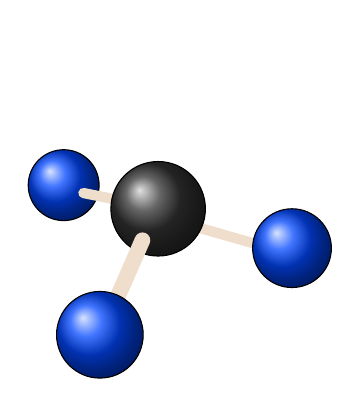
\begin{tikzpicture}[line join=round, line cap=round,scale=1,transform shape] 
        \definecolor{blue(ryb)}{rgb}{0.01, 0.28, 1.0}
        \definecolor{anti-flashwhite}{rgb}{0.95, 0.95, 0.96}
        \definecolor{almond}{rgb}{0.94, 0.87, 0.8}
        \tikzset{phan_tu/.pic={
                \def\a{1}
                \def\b{.45}
                \def\c{.6}
                \def\d{.5}
                \def\e{.55}
                \path
                (0,2) coordinate (A)
                (-1.25,0) coordinate (B)
                (-.05,-.3) coordinate (C)
                (1.65,-.8) coordinate (D)
                (-0.79,-1.9) coordinate (E)
                ; 
                \draw[almond,line width=1.3mm] (.5,-.55)--(1.2,-.75);
                \draw[ball color=blue(ryb)] (B) circle (\b);
                \draw[almond,line width=1.3mm] (-1,-.1)--(-.5,-.2);
                \draw[ball color=black!80] (C) circle (\c);
                %\draw[almond,line width=2mm] (-.1,1)--(-.1,.2);
                %\draw[ball color=blue(ryb)] (A) circle (\a);
                \draw[almond,line width=2mm] (-.6,-1.5)--(-.25,-.7);
                \draw[ball color=blue(ryb)] (D) circle (\d);
                \draw[ball color=blue(ryb)] (E) circle (\e);
        }} 
        \path
        (0,0)pic[scale=1]{phan_tu}; 
        \end{tikzpicture}
        \begin{tikzpicture}[>=stealth,line join=round,line cap=round,line width=1pt,scale=3.5, font=\footnotesize]
            
            \draw (0,0)coordinate(H1)--(-35:0.8)coordinate(H2)--(1,0)coordinate(H3);
            \draw[dashed,black]  ($(H2)!.5!(H3)$)coordinate(M1)--($(H1)!2/3!(M1)$)coordinate(H)--(H1)--(H3) (H)--($(H)+(90:1)$)coordinate(N);
            \draw[black,scale=2.5] (H1)node[left]{$H_1$}--(N)node[right]{$N$}--(H3)node[right]{$H_3$} (N)--(H2)node[below]{$H_2$};
            \draw[red,->] (H)node[below]{$O$}--($(H)+(90:1.2)$)node[right]{$z$};
            \draw[red,->] (H)--($4*(M1)-4*(H)$)node[above]{$y$};
            \draw[red,->] (H)--($(H2)-(H3)+(H)$)node[above]{$x$};
            \path       (intersection of H1--H and H2--H3)  coordinate (M);
            \draw (M)+(20:1 mm)node[font=\footnotesize] {$M$};
            \foreach \diem in {N,H1,H2,H3,H}\fill (\diem)circle(0.5pt);
        \end{tikzpicture}
    \end{center}
    \loigiai{
        Gọi $y$ là khoảng cách giữa nguyên tử nitrogen với mỗi nguyên tử hydrogen; khi đó $NH_2=y$.\\
        Vì $H_1(0;-2;0)$ nên 
        $$  O H_1=2 \Rightarrow M H_1=\frac{3}{2} O H_1=3 \Rightarrow H_1 H_2=H_2 H_3=H_3 H_1=\dfrac{M H_1}{\dfrac{\sqrt{3}}{2}}=2 \sqrt{3}.$$
        Áp dụng định lí cosin ta có $$ H_1H_2^2=NH_1^2+NH_2^2-2\cdot NH_1\cdot NH_2\cdot\cos \widehat{H_1NH_2}\Leftrightarrow 2y^2-2y^2\cos 107^\circ=12$$ $$\Leftrightarrow y^2=\dfrac{12}{2-2\cos 107^\circ}\Leftrightarrow y\approx 2{,}15.$$
		Vậy khoảng cách ngắn nhất giữa các nguyên tử là $2{,}15$.
        }
\end{ex}

\begin{ex}%[2H2H2-3]%[Dự án dề cương 3 Khối NH24-25-Đợt 2-Nguyễn Thanh Phong]
	Trong không gian $Oxyz$, cho các điểm $A(0;-2;-1)$, $B(1;-1;2)$. Điểm $M(a;b;c)$ trên đoạn $AB$ sao cho $MA = 2MB$. Tính $3a+3b+c$.
\loigiai{
\begin{itemize}
    \item Gọi tọa độ điểm $M(x_M; y_M; z_M)$. Vì $MA = 2MB \Rightarrow \overrightarrow{AM} = 2\overrightarrow{MB}. \quad (*)$
    \item Ta có $\overrightarrow{AM} = (x_M; y_M+2; z_M-1)$, $2\overrightarrow{MB} = 2(1-x_M; -1-y_M; 2-z_M) = (2-2x_M; -2-2y_M; 4-2z_M)$.
 $$(*) \Leftrightarrow \heva{&x = 2-2x \\&y+2 = -2-2y \\&z-1 = 4-2z } \Leftrightarrow \heva{&x = \dfrac{2}{3} \\&y = \dfrac{-4}{3} \\&z = 1.}$$
    \item Suy ra tọa độ điểm $M$ là $\left(\dfrac{2}{3}; \dfrac{-4}{3}; 1\right)$. Do đó: $3a+3b+c = -1$.
\end{itemize}
}
\end{ex}

